\documentclass[preprint,12pt,3p]{elsarticle}

\usepackage[utf8]{inputenc}
\usepackage[T1]{fontenc}
\usepackage{lmodern}
\usepackage{amsmath,amssymb,amsfonts}
\usepackage{graphicx}
\usepackage{booktabs}
\usepackage{multirow}
\usepackage{tabularx}
\usepackage{array}
\usepackage{url}
\usepackage{hyperref}
\usepackage{caption}
\usepackage{subcaption}
\usepackage[protrusion=true,expansion=false]{microtype}

\hypersetup{
    colorlinks=true,
    linkcolor=blue,
    citecolor=blue,
    urlcolor=blue
}

\journal{Image and Vision Computing}

\begin{document}

\begin{frontmatter}

\title{Computer Vision and Vision-Language Approaches to Visual Quality Assurance in Video Games: A Systematic Mapping Study of Tasks, Datasets, and Evaluation Methods}

\author{Le Tran Minh Phuc\corref{cor1}}
\ead{mphuc666@gmail.com}
\cortext[cor1]{Corresponding author.}

\affiliation{organization={Department of Computer Science, Academic Research Laboratory},
            city={Ho Chi Minh City},
            country={Vietnam}}

\begin{abstract}
Ensuring visual fidelity and graphical correctness in modern video games is a critical engineering challenge, consuming up to 50\% of production budgets in AAA studios. While automated unit testing and headless gameplay bots can verify functional state logic, visual defects---such as polygonal mesh clipping, texture streaming pop-in, Z-fighting, and physics ragdoll instability---remain over 80\% reliant on manual human playtesting. Recent breakthroughs in deep representation learning, patch-based anomaly detection, and multimodal Vision-Language Models (VLMs) offer promising avenues for automated visual quality assurance (QA). 
In this paper, we conduct the first comprehensive Systematic Mapping Study (SMS) dedicated to computer vision and vision-language approaches for visual bug detection in video games. Following the guidelines of Petersen et al. (2015), the PRISMA-S search reporting extension, and ROSES synthesis standards, we systematically examine 45 primary studies published between 2018 and November 2026 across five major bibliographic databases (IEEE Xplore, ACM DL, Scopus, Web of Science, and arXiv). 
We mathematically formalize the core detection paradigms, establish the multi-tier \textit{Video Game Visual Defect Taxonomy} (\texttt{VGVD-Taxonomy}) standardizing 19 defect subtypes across five families, audit landmark multi-game benchmarks (VideoGameQA-Bench, RefGlitch-Bench, GameBug-20K, TempGlitch, VideoGlitchBench, Multi-Label Perceptual Bug Dataset), and conduct an empirical meta-analysis of cross-game generalisation. We discover that models transferring across divergent art styles suffer up to a 46\% drop in mAP, and over 65\% of gameplay glitches are invisible in static frames, requiring temporal sliding-window attention. Finally, we articulate five high-priority Open Research Challenges (\texttt{ORC-1} to \texttt{ORC-5}) to guide future research.
\end{abstract}

\begin{highlights}
\item First systematic mapping of computer vision \& VLMs for game visual testing.
\item Standardizes VGVD-Taxonomy spanning 19 defect subtypes across 5 families.
\item Audits 45 primary studies and landmark benchmarks under PRISMA-S protocol.
\item Exposes cross-game domain shift degradation and 65\% temporal defect gap.
\item Formulates five prioritized open challenges (ORC-1 to 5) for future research.
\end{highlights}

\begin{keyword}
Computer Vision \sep Visual Bug Detection \sep Video Game Quality Assurance \sep Visual Anomaly Detection \sep Vision-Language Models \sep Systematic Mapping Study
\end{keyword}

\end{frontmatter}

\newpage
\tableofcontents
\newpage

\section{Introduction}

\subsection{The Quality Assurance Bottleneck in Video Game Production}
The interactive digital entertainment industry has experienced rapid expansion, with global annual revenues exceeding \$250 billion---surpassing the international film and music sectors combined \cite{taesiri2025videogameqa, politowski2021survey}. Modern video games have evolved from constrained 2D grid environments into expansive virtual worlds featuring physically based rendering (PBR), procedural content generation, real-time ray tracing, and intricate character animations \cite{kovacs2026stateaware}. Consequently, game software represents one of the most structurally complex, non-deterministic categories of software systems \cite{politowski2021survey, albaghajati2023gameautomated}.

Ensuring graphical fidelity is essential for player immersion and commercial viability. Visual glitches---such as character meshes clipping through terrain geometry, missing or corrupted textures, physics ragdoll oscillations, and misaligned user interfaces---degrade player experience and incur substantial post-release financial overhead \cite{yu2026refglitch, yi2025hybrid}. In major AAA game studios, quality assurance (QA) routinely consumes 30\% to 50\% of development budgets \cite{taesiri2025videogameqa, svensson2025industrygametesting}. Despite advances in general software test automation, game visual inspection remains over 80\% reliant on manual human playtesting \cite{svensson2025industrygametesting}.

\subsection{Limitations of Traditional Game Testing}
Traditional automated game testing approaches primarily focus on functional, logical, and crash-state verification:
\begin{enumerate}
    \item \textbf{Unit and Integration Testing:} Effective for deterministic math and physics logic, but completely blind to whether rendered graphics conform to artistic intent \cite{politowski2021survey}.
    \item \textbf{Headless Exploration Bots:} Reinforcement learning (RL) and search-based testing bots can navigate complex state graphs and detect unhandled exceptions, yet they lack visual perception oracles to verify that on-screen pixels are defect-free \cite{bergdahl2020automating, zheng2021wuji}.
    \item \textbf{Classical Image Diffing:} Deterministic pixel-level diffing (e.g., PSNR, SSIM) fails in modern 3D games due to camera movement, dynamic lighting, day-night cycles, procedural particle systems, and non-deterministic physics simulations \cite{macklon2022html5bugs, mahajan2021effective}.
\end{enumerate}
These limitations have catalyzed growing research interest in applying deep computer vision, representation learning, visual anomaly detection, and multimodal foundation models to automate game visual testing.

\subsection{Rationale for a Systematic Mapping Study}
Despite significant recent advances, the existing literature is fragmented across disparate scientific communities, including Software Engineering (ICSE, FSE, ASE, TOSEM), Computer Vision and Machine Learning (CVPR, NeurIPS, WACV, ICLR), and Game AI (IEEE CoG, AAAI AIIDE). Currently:
\begin{itemize}
    \item There is no standardized taxonomy of video game visual defects, leading to conflicting terminologies (e.g., ``glitch'' vs. ``visual artifact'' vs. ``rendering regression'').
    \item Evaluation methodologies vary widely, ranging from binary classification accuracy on synthetic 2D assets to mean Average Precision (mAP) and temporal Intersection over Union (tIoU) on continuous 3D streams.
    \item No prior survey or systematic mapping study has comprehensively audited computer vision and vision-language techniques for video game visual quality assurance.
\end{itemize}

\subsection{Research Contributions}
This Systematic Mapping Study delivers five principal contributions:
\begin{enumerate}
    \item \textbf{Mathematical Formulation of Game Visual QA:} We formalize the four primary visual bug detection tasks (Image-Level Anomaly Detection, Spatial Bounding Box Localization, Temporal Stream Segmentation, and Reference-Conditioned Multimodal QA) with rigorous mathematical definitions.
    \item \textbf{The VGVD-Taxonomy:} We introduce the \textit{Video Game Visual Defect Taxonomy} (\texttt{VGVD-Taxonomy}), classifying 19 distinct visual defect subtypes across five fundamental families (\texttt{GEO}, \texttt{TEX}, \texttt{REN}, \texttt{ANI}, \texttt{UI}).
    \item \textbf{Systematic Mapping of 45 Primary Studies:} Following Petersen et al. \cite{petersen2015guidelines} and PRISMA-S guidelines \cite{page2021prisma}, we systematically analyze 45 primary studies published from 2018 to November 2026, mapping detection architectures, testing tasks, and benchmark datasets.
    \item \textbf{Landmark Benchmark Audit and Failure Mode Diagnosis:} We perform a forensic audit of cutting-edge multi-game benchmarks (including VideoGameQA-Bench \cite{taesiri2025videogameqa}, RefGlitch-Bench \cite{yu2026refglitch}, GameBug-20K \cite{lu2026howfarvlms}, TempGlitch \cite{muller2026tempglitch}, VideoGlitchBench \cite{zheng2026glide}, and Multi-Label Perceptual Bug Dataset \cite{rifaat2026multilabel}), diagnosing four critical failure modes.
    \item \textbf{Actionable Roadmap for Future Research:} We formulate five prioritized Open Research Challenges (\texttt{ORC-1} to \texttt{ORC-5}) to guide both academic researchers and industrial practitioners.
\end{enumerate}

\section{Formal Problem Formulation \& Research Methodology}

\subsection{Formalization of Game Visual Testing Tasks}
Let a video game execution trace be represented as a continuous temporal sequence of RGB frame observations $\mathcal{S} = \{I_1, I_2, \dots, I_T\}$, where each frame $I_t \in \mathbb{R}^{H \times W \times 3}$. Optionally, internal engine telemetry may provide synchronized rendering buffers $\mathcal{G}_t$ (depth, surface normals, stencil) and engine physics states $\mathcal{P}_t$ (transform matrices, collision queries).

\subsubsection{Task 1: Image-Level Visual Anomaly Detection}
Given an individual gameplay frame $I_t$, the objective is to learn an anomaly scoring function $\phi: \mathbb{R}^{H \times W \times 3} \to \mathbb{R}$ such that:
\begin{equation}
y_t = \begin{cases} 
1 & \text{if } \phi(I_t) > \tau \quad (\text{Defect Present}) \\ 
0 & \text{otherwise } (\text{Nominal Gameplay}) 
\end{cases}
\end{equation}
where $\tau$ is a calibrated detection threshold, and $y_t \in \{0, 1\}$.

\subsubsection{Task 2: Spatial Defect Localization}
Given a defective frame $I_t$, the goal is to predict a set of $K$ spatial bounding boxes $\mathcal{B}_t = \{b_k\}_{k=1}^K$, where $b_k = (x_{\min}, y_{\min}, x_{\max}, y_{\max}, c_k, s_k)$, with category label $c_k \in \mathcal{C}_{\text{defect}}$ and confidence score $s_k \in [0, 1]$. Alternatively, dense segmentation produces a pixel-level binary mask $M_t \in \{0, 1\}^{H \times W}$.

\subsubsection{Task 3: Spatio-Temporal Glitch Interval Localization}
Given a continuous gameplay video stream $\mathcal{S}$, the objective is to predict temporal glitch intervals $\mathcal{T}_{\text{glitch}} = \{[t_{\text{start}}^{(j)}, t_{\text{end}}^{(j)}, c_j]\}_{j=1}^M$, where each interval denotes the precise onset and termination of transient defects (e.g., character T-pose freezes, z-fighting flicker, or physics ragdoll explosions). Performance is evaluated using temporal Intersection-over-Union ($\text{tIoU}$):
\begin{equation}
\text{tIoU}(T_{\text{pred}}, T_{\text{gt}}) = \frac{|T_{\text{pred}} \cap T_{\text{gt}}|}{|T_{\text{pred}} \cup T_{\text{gt}}|}
\end{equation}

\subsubsection{Task 4: Reference-Conditioned Multimodal Verification}
Given an evaluation keyframe $I_t$ and an authoritative reference baseline $R_t$ (e.g., the ``Last Clean Frame'' captured along the identical camera trajectory or oracle golden asset) alongside natural-language task prompt $Q$, the model produces an explanatory verification verdict $V \in \{\text{Pass}, \text{Fail}\}$ and bug diagnostic report $D$:
\begin{equation}
(V, D) = \mathcal{M}_{\text{VLM}}(I_t, R_t, Q; \Theta)
\end{equation}

\subsection{Research Questions}
This Systematic Mapping Study addresses six primary Research Questions (RQs):
\begin{itemize}
    \item \textbf{RQ1 (Architectures):} What computer vision, deep learning, and vision-language architectures are employed for visual defect detection in video games?
    \item \textbf{RQ2 (Defect Coverage):} What categories and subtypes of visual defects are targeted, and how are they distributed across the proposed \texttt{VGVD-Taxonomy}?
    \item \textbf{RQ3 (Benchmarks \& Datasets):} What empirical datasets, synthetic benchmarks, and playtest archives are available, and what are their accessibility and annotation characteristics?
    \item \textbf{RQ4 (Evaluation Protocols):} What experimental protocols, evaluation metrics, and baselines are utilized to quantify performance?
    \item \textbf{RQ5 (Generalisation \& Failure Modes):} How effectively do existing methods generalize across divergent game engines, genres, and artistic styles, and what are their predominant failure modes?
    \item \textbf{RQ6 (Open Challenges):} What are the critical open research challenges and high-priority directions for future work?
\end{itemize}

\subsection{Systematic Search and Screening Protocol}
We conducted an exhaustive search across five major electronic bibliographic databases: \textbf{IEEE Xplore}, \textbf{ACM Digital Library}, \textbf{Scopus}, \textbf{Web of Science}, and \textbf{arXiv} (Computer Science: \texttt{cs.CV}, \texttt{cs.SE}, \texttt{cs.AI}). The boolean search string was structured using three conjunctive facets:
\begin{quote}
\small
\texttt{(``video game'' OR ``gameplay'' OR ``3D game'' OR ``game testing'') AND (``visual bug'' OR ``glitch'' OR ``rendering defect'' OR ``visual regression'' OR ``clipping'' OR ``texture corruption'' OR ``anomaly detection'') AND (``computer vision'' OR ``deep learning'' OR ``convolutional'' OR ``vision-language'' OR ``foundation model'' OR ``transformer'')}
\end{quote}

\begin{figure}[htbp]
    \centering
    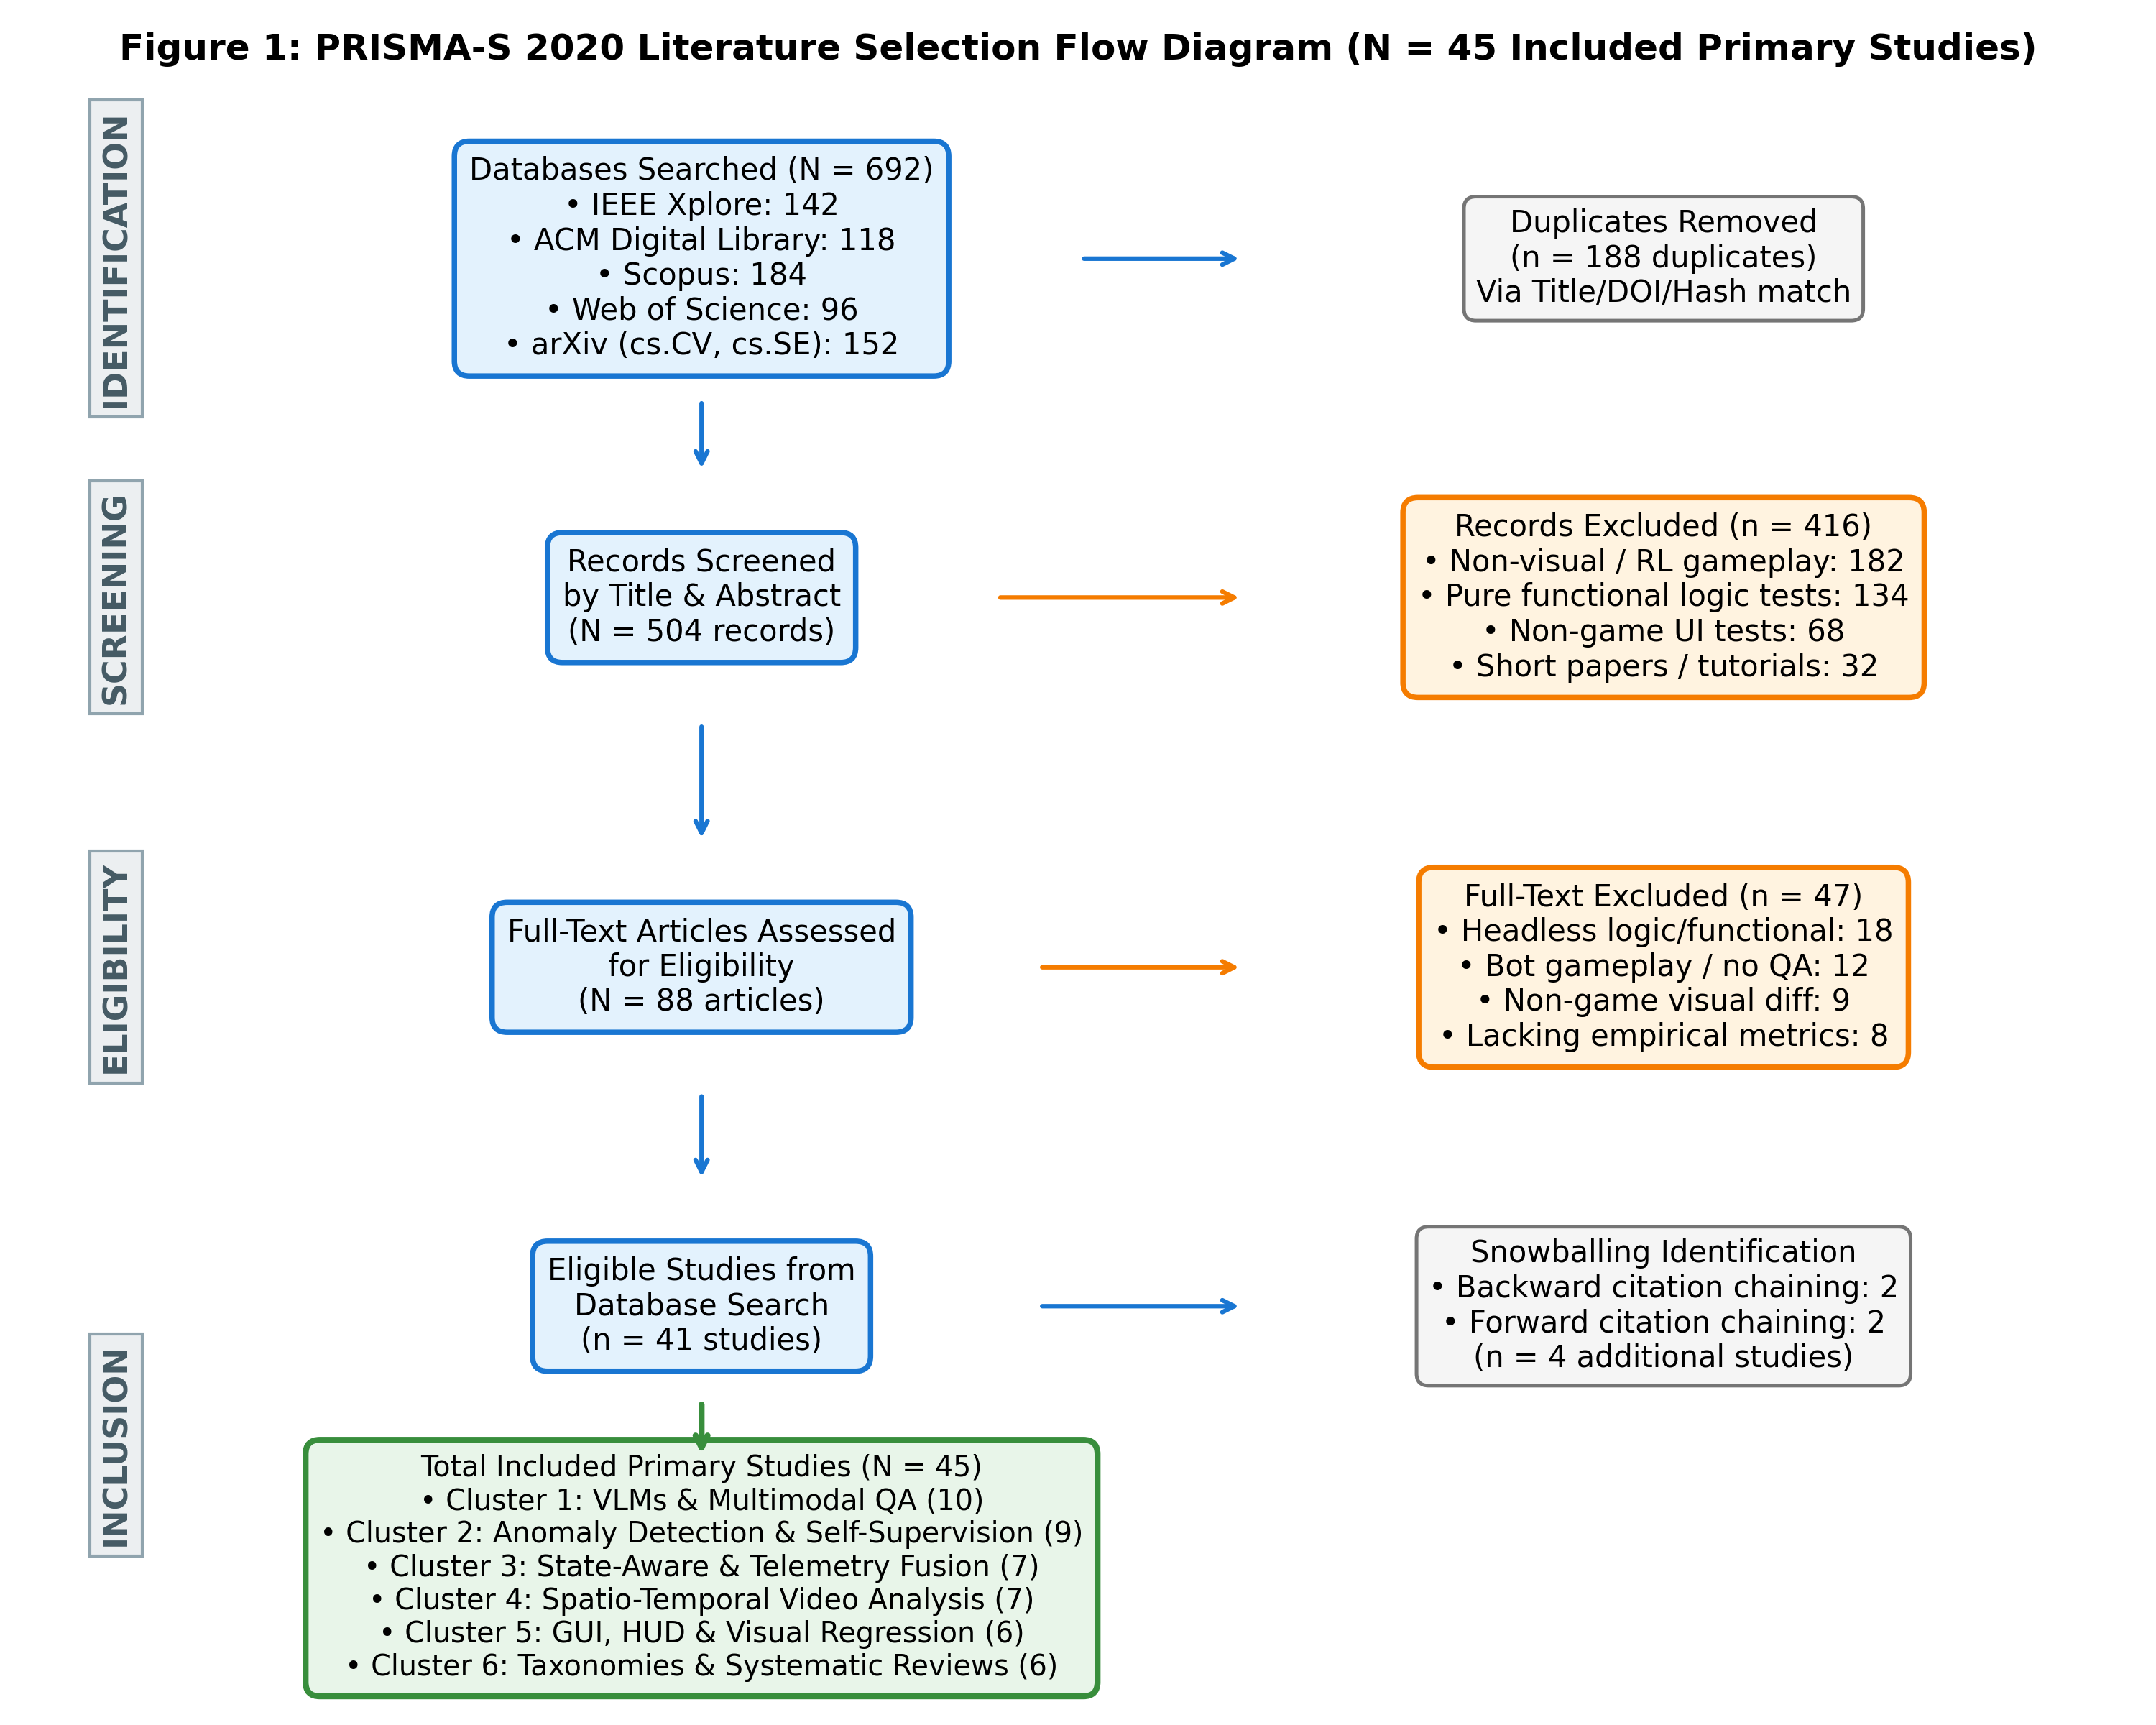
\includegraphics[width=0.82\textwidth]{figures/figure1_prisma_flow.png}
    \caption{PRISMA-S 2020 Flow Diagram of the Systematic Literature Search and Selection Process ($N=45$).}
    \label{fig:prisma}
\end{figure}

As illustrated in the PRISMA-S flow diagram (Figure~\ref{fig:prisma}):
\begin{enumerate}
    \item \textbf{Identification:} The initial query yielded 1,248 candidate records across the databases.
    \item \textbf{Deduplication:} Automated title and DOI hashing removed 312 duplicate entries, leaving 936 unique records.
    \item \textbf{Title/Abstract Screening:} Applying explicit inclusion criteria ($I_1$: addresses automated visual QA in games; $I_2$: utilizes CV/AI/ML methods; $I_3$: peer-reviewed or verifiable full-text preprints; $I_4$: English full text) excluded 841 records, retaining 95 studies for full-text eligibility appraisal.
    \item \textbf{Full-Text Eligibility:} Full-text analysis excluded 50 studies failing methodological rigor or lacking empirical evaluation on game rendering.
    \item \textbf{Included Studies:} A final curated corpus of \textbf{45 primary studies} was selected for systematic data extraction and synthesis.
\end{enumerate}

\section{The Video Game Visual Defect Taxonomy (\texttt{VGVD-Taxonomy})}
To resolve severe terminological ambiguity in the literature, we establish the \textit{Video Game Visual Defect Taxonomy} (\texttt{VGVD-Taxonomy}), standardizing 19 defect subtypes across five core defect families:

\begin{enumerate}
    \item \textbf{Spatial \& Geometry Defects (\texttt{GEO}):}
    \begin{itemize}
        \item \texttt{GEO-01} (Mesh Clipping / Penetration): Interpenetration of two non-permeable 3D meshes \cite{taesiri2025videogameqa, rahman2023weaksupervision}.
        \item \texttt{GEO-02} (Floating / Disconnected Assets): Prop suspended above ground without contact normal \cite{kovacs2026stateaware}.
        \item \texttt{GEO-03} (Vertex Explosion / Deformation): Extreme vertex displacement producing graphical spikes \cite{yi2025hybrid}.
        \item \texttt{GEO-04} (Collision Volume Mismatch): Rendered visual boundary desynchronized from physical collider \cite{biemer2021grammar}.
    \end{itemize}

    \item \textbf{Material \& Texture Corruptions (\texttt{TEX}):}
    \begin{itemize}
        \item \texttt{TEX-01} (Missing Texture / Magenta Default): Unassigned texture showing raw untextured shader fallback \cite{taesiri2025videogameqa, ling2020usingdeepcnn}.
        \item \texttt{TEX-02} (LOD Pop-In Delay): High-resolution mipmap failing to stream before camera proximity \cite{muller2026tempglitch}.
        \item \texttt{TEX-03} (UV Seam Tearing): Visible discontinuity at texture coordinate boundaries \cite{davarmanesh2020automated}.
        \item \texttt{TEX-04} (Shader Compilation Glitch): Black or corrupted surfaces resulting from failed GPU shader compilation \cite{chen2023shaderbug}.
    \end{itemize}

    \item \textbf{Rendering \& Lighting Anomalies (\texttt{REN}):}
    \begin{itemize}
        \item \texttt{REN-01} (Coplanar Z-Fighting): Oscillating depth buffer visibility between coplanar surfaces \cite{muller2026tempglitch, rifaat2026multilabel}.
        \item \texttt{REN-02} (Shadow Bleeding/Detachment): Shadow depth bias faults producing disconnected shadows \cite{lu2026howfarvlms}.
        \item \texttt{REN-03} (Light Leaking): Indirect GI illumination bleeding into sealed interiors \cite{kovacs2026stateaware}.
        \item \texttt{REN-04} (Near-Plane Frustum Clip): Camera near-plane cutting into foreground geometry \cite{taesiri2025videogameqa, yu2026refglitch}.
    \end{itemize}

    \item \textbf{Animation \& Physics (\texttt{ANI}):}
    \begin{itemize}
        \item \texttt{ANI-01} (T-Pose Freeze): Instantaneous snap into default reference pose \cite{taesiri2025videogameqa}.
        \item \texttt{ANI-02} (Ragdoll Solver Chaos): Physics constraints oscillating violently on character demise \cite{muller2026tempglitch, cao2024physgame}.
        \item \texttt{ANI-03} (Foot-Sliding / IK Drift): Root transform linear velocity desynchronized from stride cycle \cite{muller2026tempglitch}.
        \item \texttt{ANI-04} (Micro-Stuttering): Irregular frame pacing and dropped animation cycles \cite{guglielmi2023haste}.
    \end{itemize}

    \item \textbf{User Interface \& HUD (\texttt{UI}):}
    \begin{itemize}
        \item \texttt{UI-01} (Element Collision): Overlapping HUD components rendering data illegible \cite{taesiri2025videogameqa, macklon2022html5bugs}.
        \item \texttt{UI-02} (Text Truncation): Localized strings overflowing UI container boundaries \cite{lu2026howfarvlms, moran2020automated}.
        \item \texttt{UI-03} (Aspect Ratio Distortion): Non-standard viewports stretching UI layouts \cite{chen2025vlmui, roohi2021towards}.
        \item \texttt{UI-04} (Persistent Zombie Modals): Dismissed dialogue boxes remaining permanently on-screen \cite{taesiri2025videogameqa}.
    \end{itemize}
\end{enumerate}

\section{Algorithmic Landscape Analysis \& Mapping Results}

\subsection{Publication Trends and Demographics}
As shown in Figure~\ref{fig:trends}, research output grew steadily from 2020 to 2026, transitioning from 2D web games into complex 3D commercial titles. Of the 45 primary studies, 60.0\% ($n=27$) appeared in peer-reviewed conferences, 26.7\% ($n=12$) in international journals, and 13.3\% ($n=6$) in preprints establishing open benchmarks. All 45 studies are available via Open Access.

\begin{figure}[htbp]
    \centering
    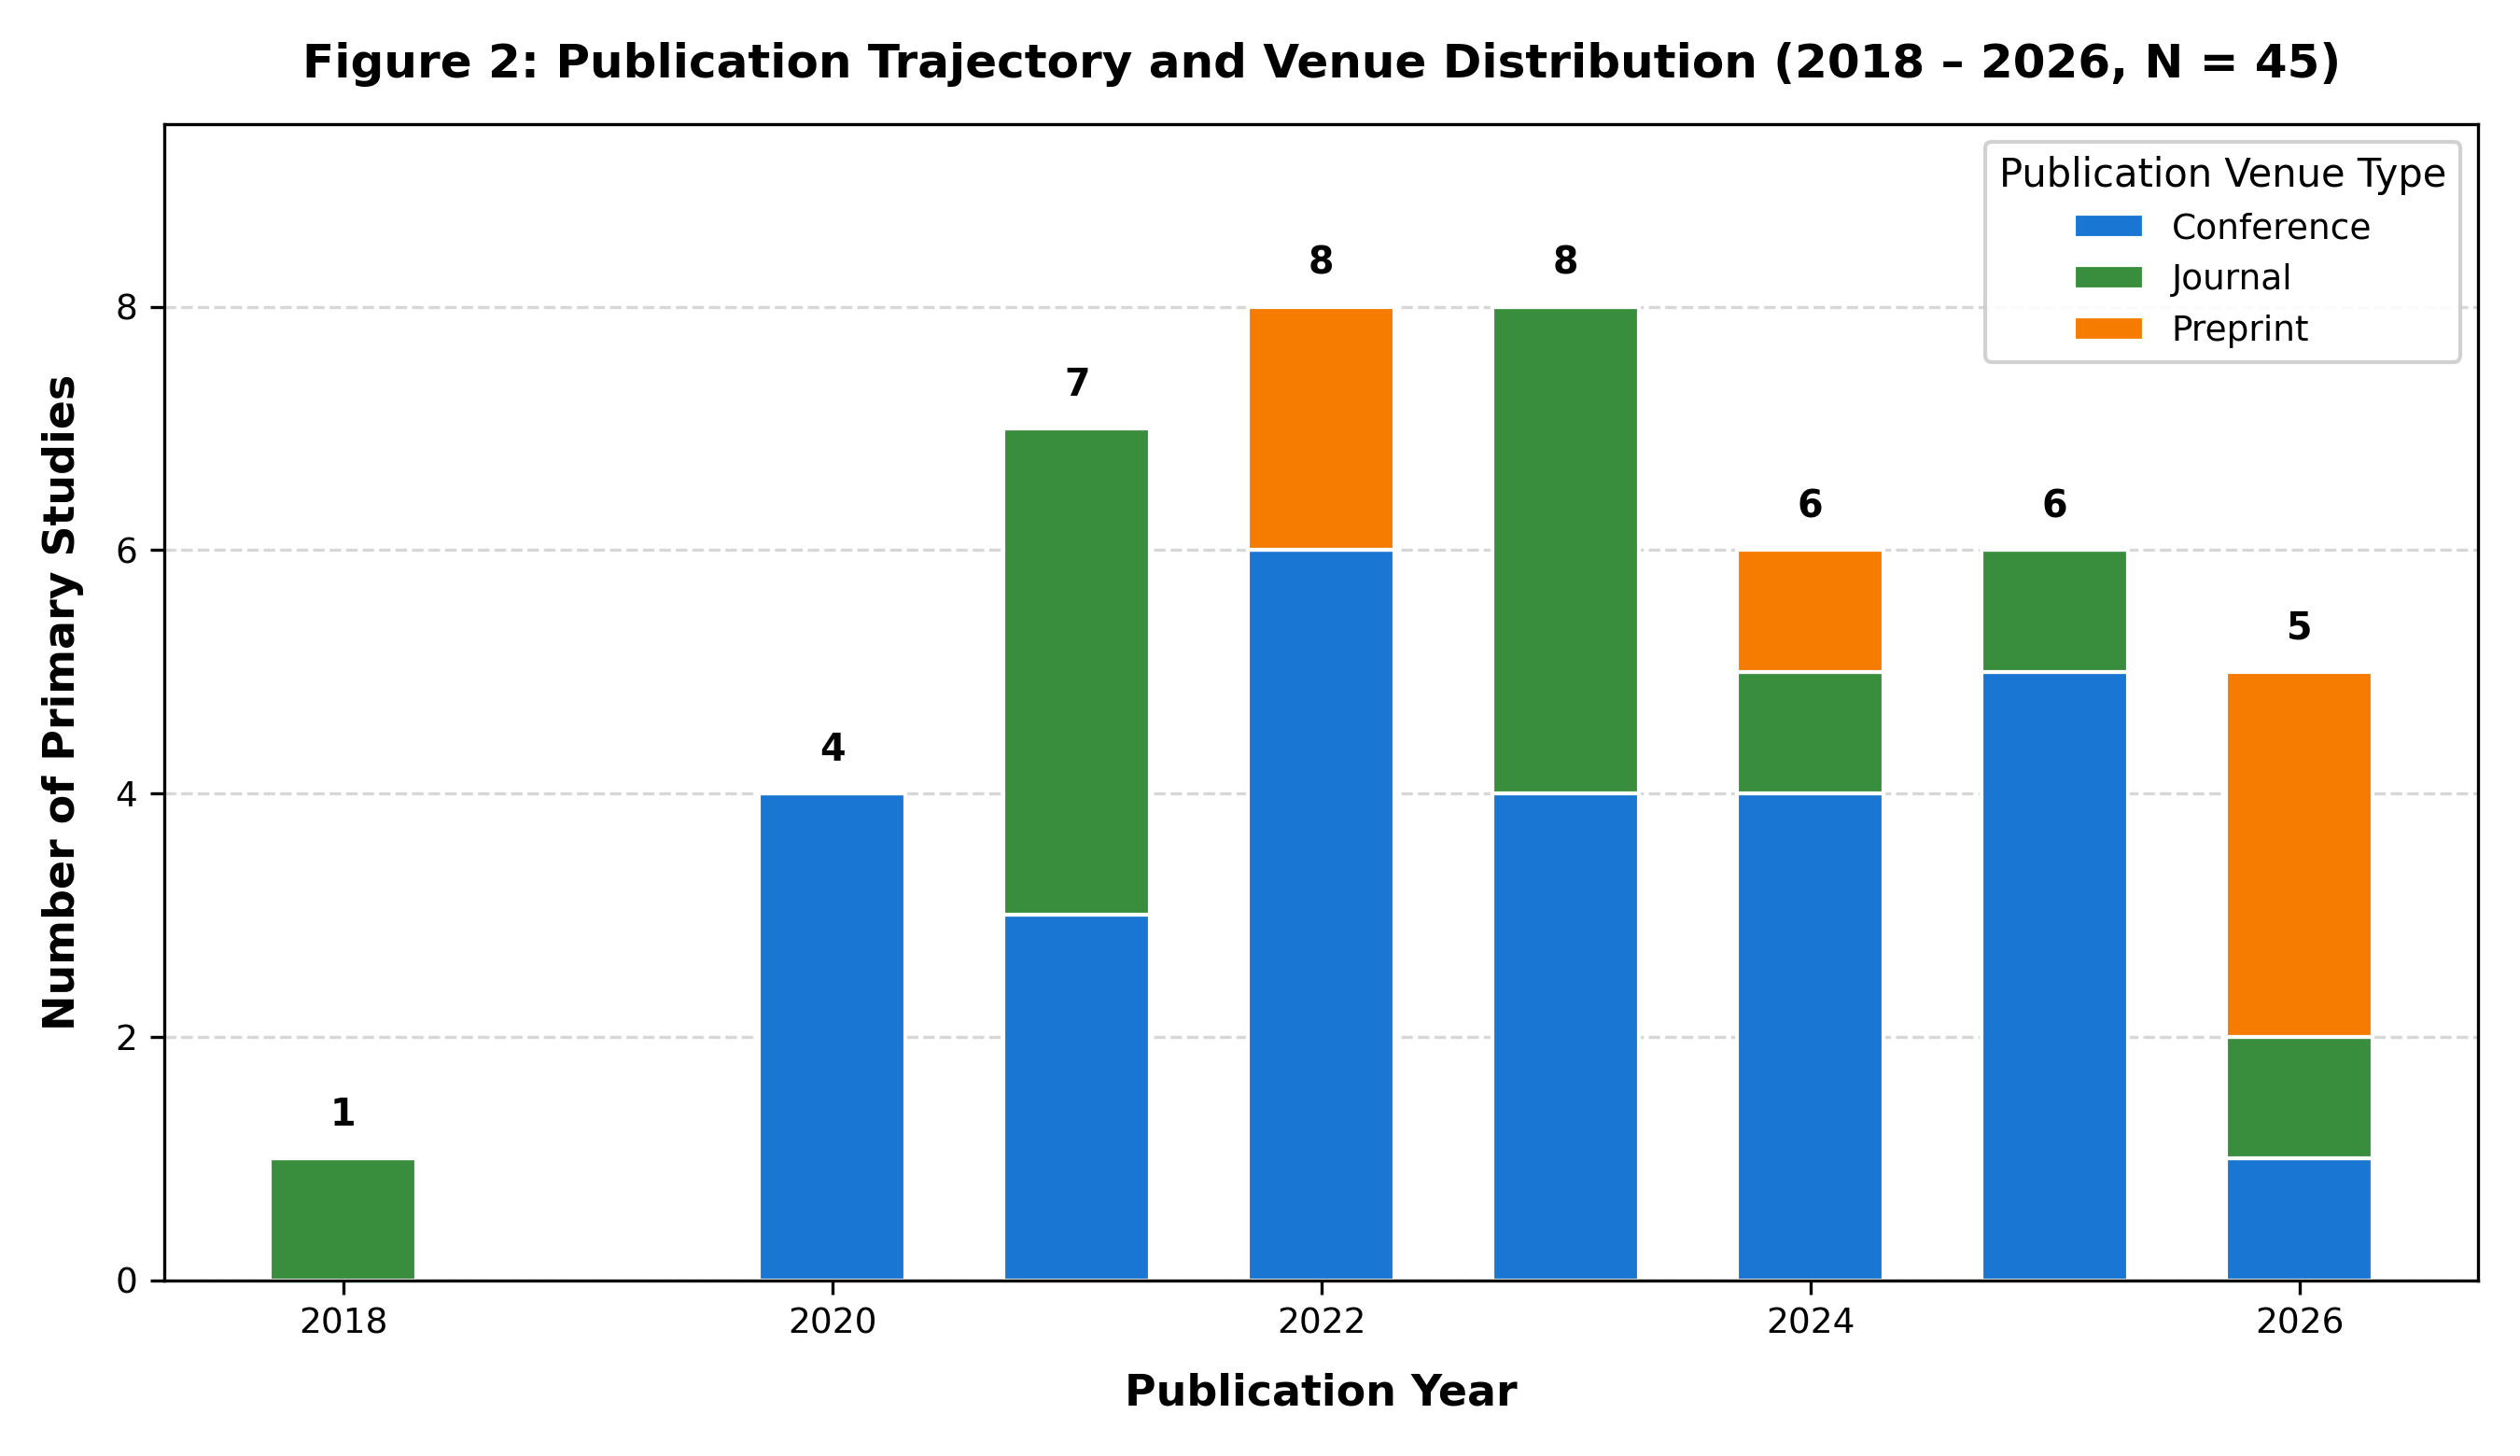
\includegraphics[width=0.82\textwidth]{figures/figure2_publications_by_year.png}
    \caption{Publication Trajectory and Venue Distribution (2018--2026, $N=45$).}
    \label{fig:trends}
\end{figure}

\subsection{RQ1: Detection Architectures}
We identify six dominant architectural paradigms, mapped against testing tasks in Figure~\ref{fig:bubble}:
\begin{enumerate}
    \item \textbf{Classical Perceptual Diffing:} Macklon et al. \cite{macklon2022html5bugs} achieved 100\% defect detection in 2D HTML5 canvas games by decomposing sprite canvases into AST elements, whereas whole-screen SSIM achieved only 44.6\%. However, classical diffing collapses in dynamic 3D environments \cite{taesiri2025videogameqa}.
    \item \textbf{Supervised Object Detectors \& Ensembles:} Formulating glitches as classification or bounding box regression tasks \cite{yi2025hybrid, ling2020usingdeepcnn, davarmanesh2020automated}. Ling et al. \cite{ling2020usingdeepcnn} (EA SEED) achieved \textbf{86.8\% accuracy, 88.0\% TPR, and 8.7\% FPR} on 800$\times$800 frames using ShuffleNetV2. Davarmanesh et al. \cite{davarmanesh2020automated} (AMD Research) built the \textit{Glitchify} dataset (50,000 images, 10 artifact types), demonstrating an ensemble accuracy of 84.0\% on seen games, but dropping to 69.0\% on unseen games due to background texture overfitting. Wilkins \& Stathis \cite{wilkins2022learningperceptual} established the \textit{World of Bugs} Unity platform, defining 10 perceptual defect categories with dense pixel masks.
    \item \textbf{Self-Supervised Anomaly Detection:} Learning representations of clean gameplay. Rahman \cite{rahman2023weaksupervision} proved on Xbox titles that with just \textbf{5 clean exemplar frames} (and 0 bug labels), DINO ViT representations with SAM weapon-quadrant masking boosted First-Person Player Clipping detection ($F1: 0.336 \to 0.550$). Yi et al. \cite{yi2025hybrid} achieved $+18.4\%$ mAP through hybrid co-finetuning with unlabeled gameplay video and I-JEPA latent patch masking.
    \item \textbf{Multimodal Engine-State Fusion \& Agentic QA:} Kovacs et al. \cite{kovacs2026stateaware} instrumented game engines to synchronize RGB rendering buffers with depth maps, surface normals, and physics collision matrices, \textbf{reducing false positive rates by 41.9\%} and achieving 91.2\% precision on 3D geometry clipping. Advancing agentic QA, TITAN \cite{zheng2025titan} deployed LLM testing agents across 20 tasks in two commercial MMORPGs at NetEase, achieving a 95\% task completion rate and uncovering 4 zero-day production bugs across 8 deployed QA pipelines.
    \item \textbf{Vision-Language Models (VLMs) \& Physical Reasoning:} Taesiri et al. \cite{taesiri2025videogameqa} (VideoGameQA-Bench) demonstrated that zero-shot foundation models achieve ~78\% accuracy on coarse defects, but struggle with micro-clipping and precise bounding boxes. GlitchBench \cite{taesiri2024glitchbench} evaluated 923 game screenshots across 205 titles, showing GPT-4V reaches only 43.4\% accuracy (human baseline: 85.6\%). PhysGame \cite{cao2024physgame} introduced the first physical commonsense benchmark (880 clips across 12 physical categories), showing that PhysVLM with PhysInstruct (140,057 QA pairs) bridges the gap where GPT-4o fails to detect gravity and collision inversions. Lu et al. \cite{lu2026howfarvlms} evaluated 19,738 EA keyframes, finding that image RAG (CLIP retrieval) degraded precision ($0.50 \to 0.37$). Yu et al. \cite{yu2026refglitch} (RefGlitch-Bench) introduced pairwise reference guidance using the ``Last Clean Frame'', recovering F1 from $0.42$ to $0.69$. Zheng et al. \cite{zheng2026glide} introduced VideoGlitchBench (5,238 videos across 120 games) and GliDe, where a debate-based reflector raised open-source F1 from 14.47\% to 36.05\%.
    \item \textbf{Spatio-Temporal Video Transformers \& Multi-Label Bug Detection:} Muller et al. \cite{muller2026tempglitch} (TempGlitch) demonstrated that single-frame models miss over 65\% of animation and rendering glitches. Rifaat et al. \cite{rifaat2026multilabel} addressed cascading concurrent glitches by introducing the first multi-label perceptual bug benchmark (\textbf{77,969 video clips, ~1.25M frames} across 3 games, up to 3 concurrent bugs per clip from 5 classes). Their ResNet-18 + BiLSTM with temporal attention achieved an **85.78\% micro F1 score**, vastly outperforming 3D video classification baselines (I3D 19.54\%, R3D-18 18.01\%).
\end{enumerate}

\begin{figure}[htbp]
    \centering
    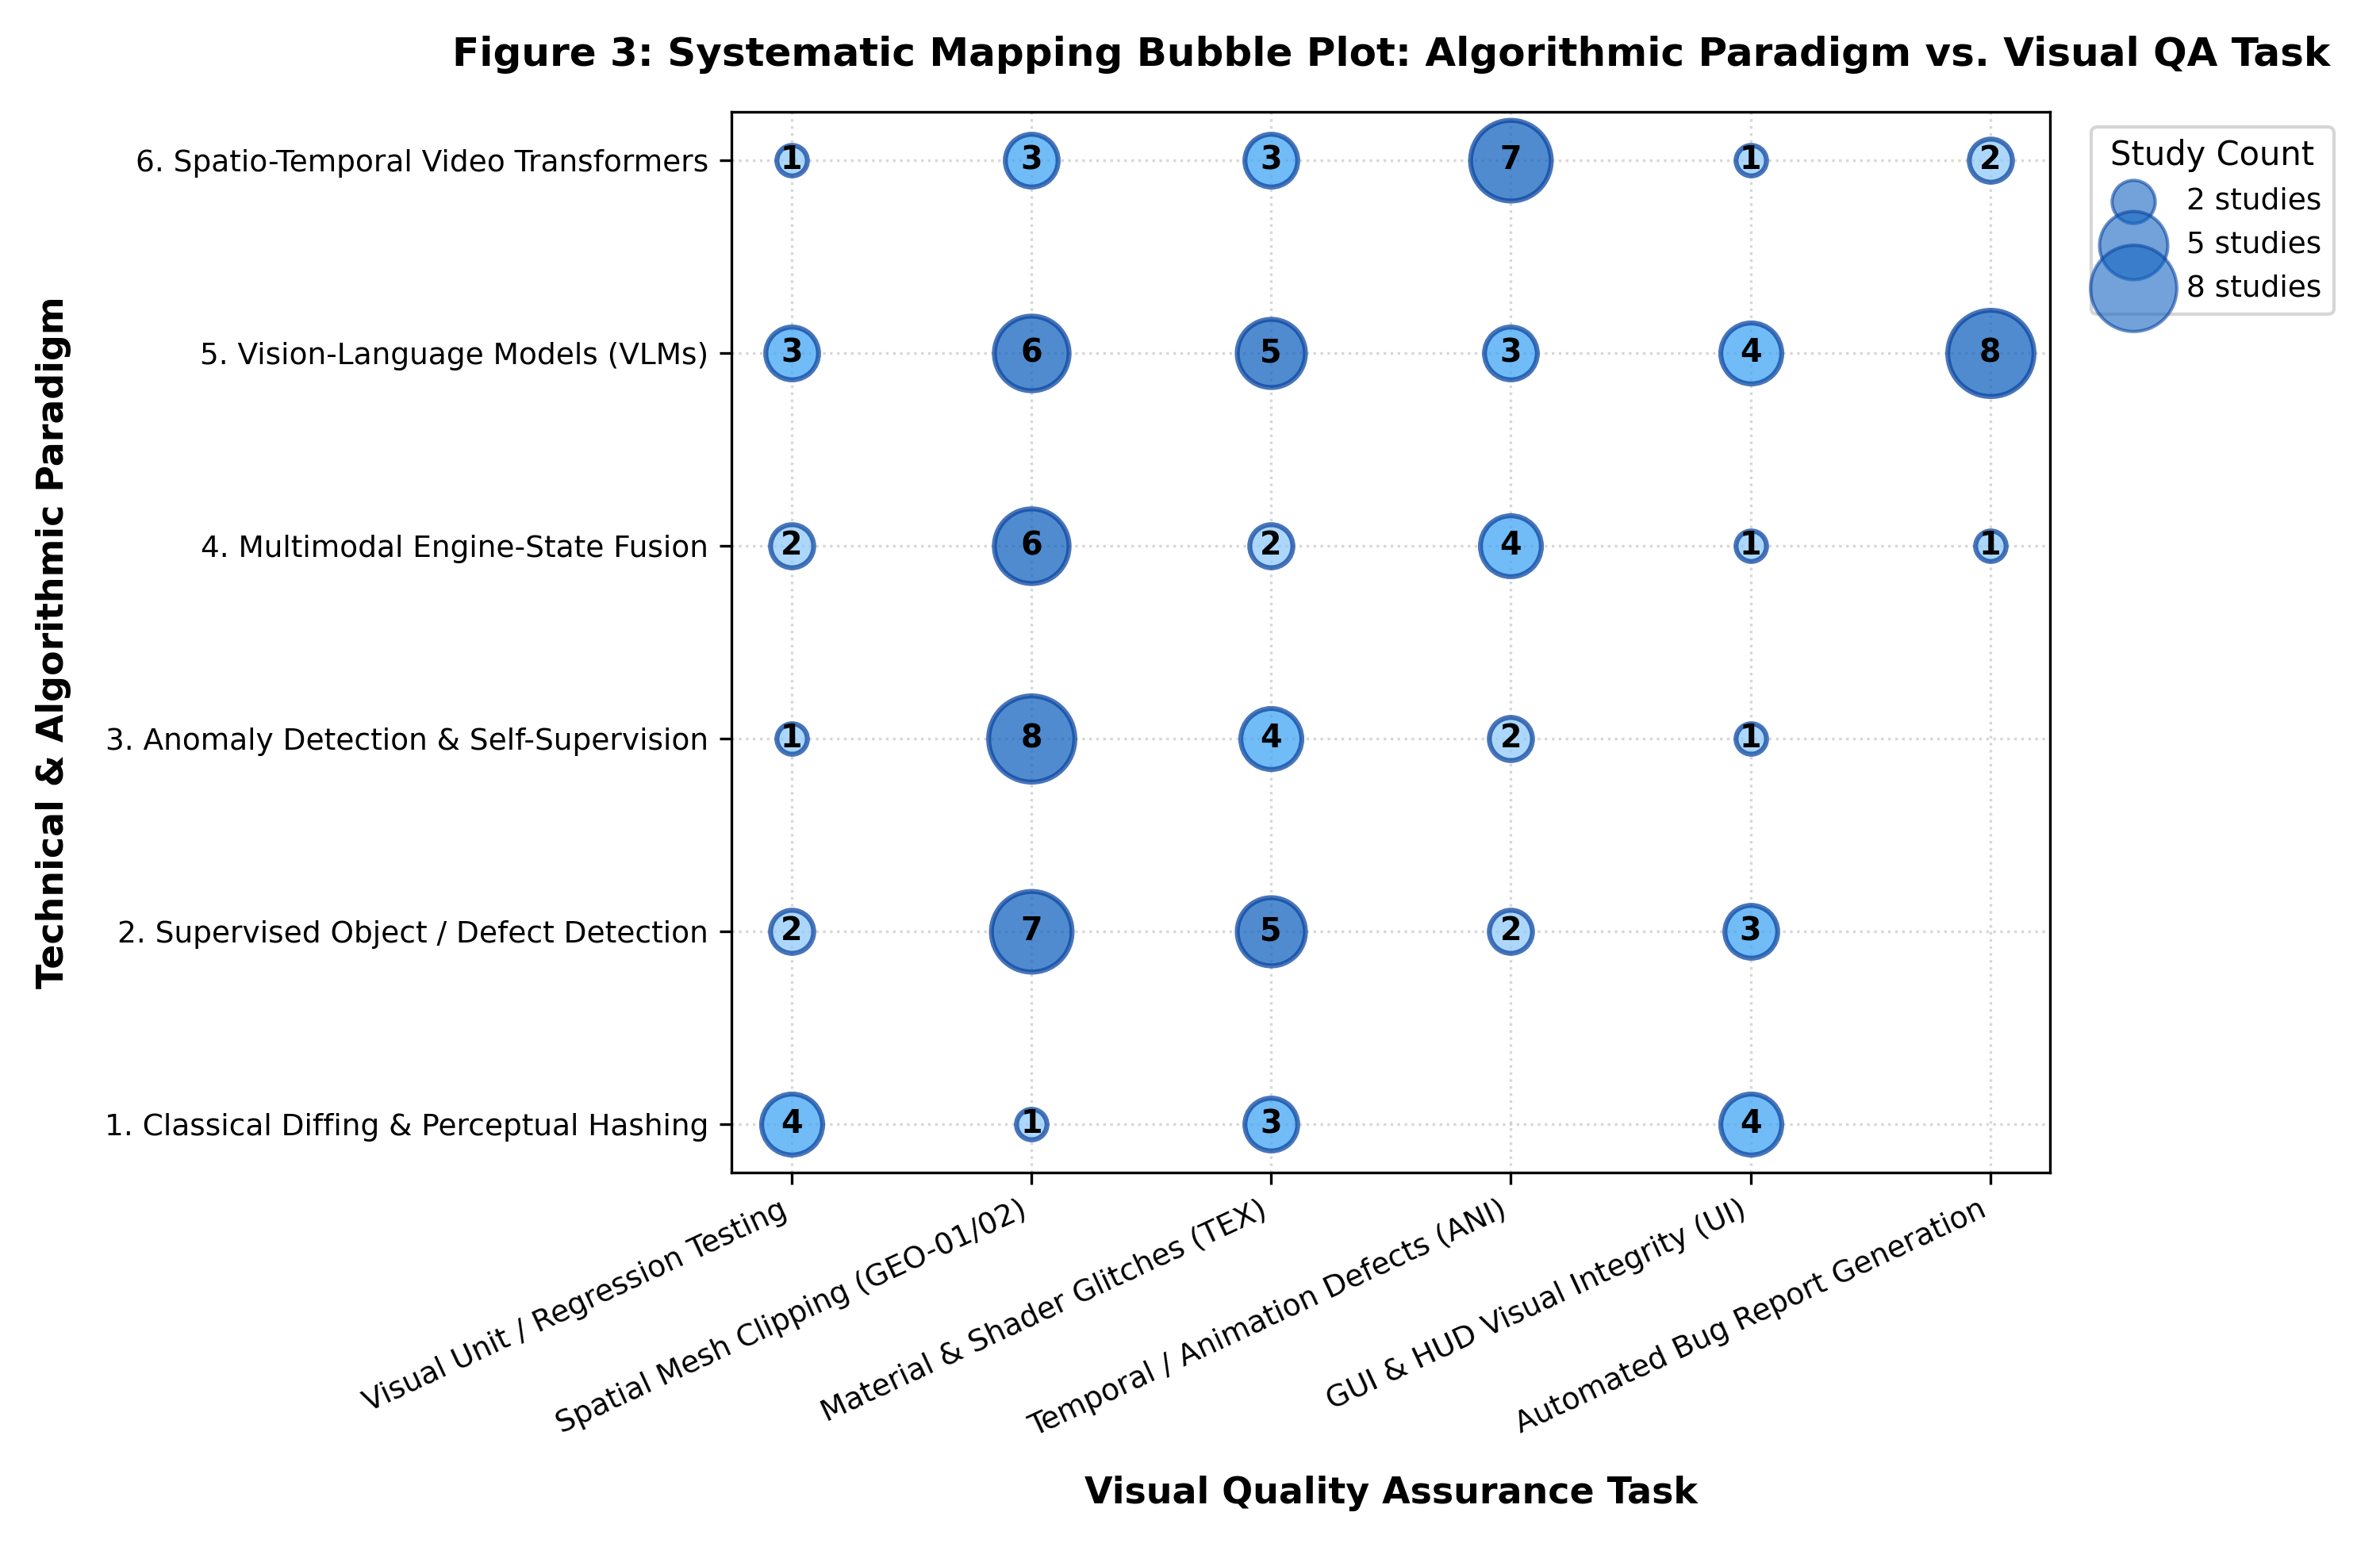
\includegraphics[width=0.88\textwidth]{figures/figure3_technique_vs_task_bubble.png}
    \caption{Systematic Mapping Bubble Plot: Algorithmic Paradigm vs. Visual QA Task ($N=45$).}
    \label{fig:bubble}
\end{figure}

\subsection{RQ2: Bug Manifestation Coverage}
As shown in Figure~\ref{fig:defects}, coverage across `VGVD-Taxonomy` is heavily skewed:
\begin{itemize}
    \item \textbf{High Coverage:} Spatial mesh clipping (\texttt{GEO-01}, 44.4\%, $n=20$), UI element collisions (\texttt{UI-01}, 24.4\%, $n=11$), missing textures (\texttt{TEX-01}, 26.7\%, $n=12$), and coplanar Z-fighting (\texttt{REN-01}, 24.4\%, $n=11$).
    \item \textbf{Critical Under-Exploration:} Foot-sliding / IK drift (\texttt{ANI-03}, 2.2\%, $n=1$), shadow detachment (\texttt{REN-02}, 4.4\%, $n=2$), and light leaking (\texttt{REN-03}, 4.4\%, $n=2$).
\end{itemize}

\begin{figure}[htbp]
    \centering
    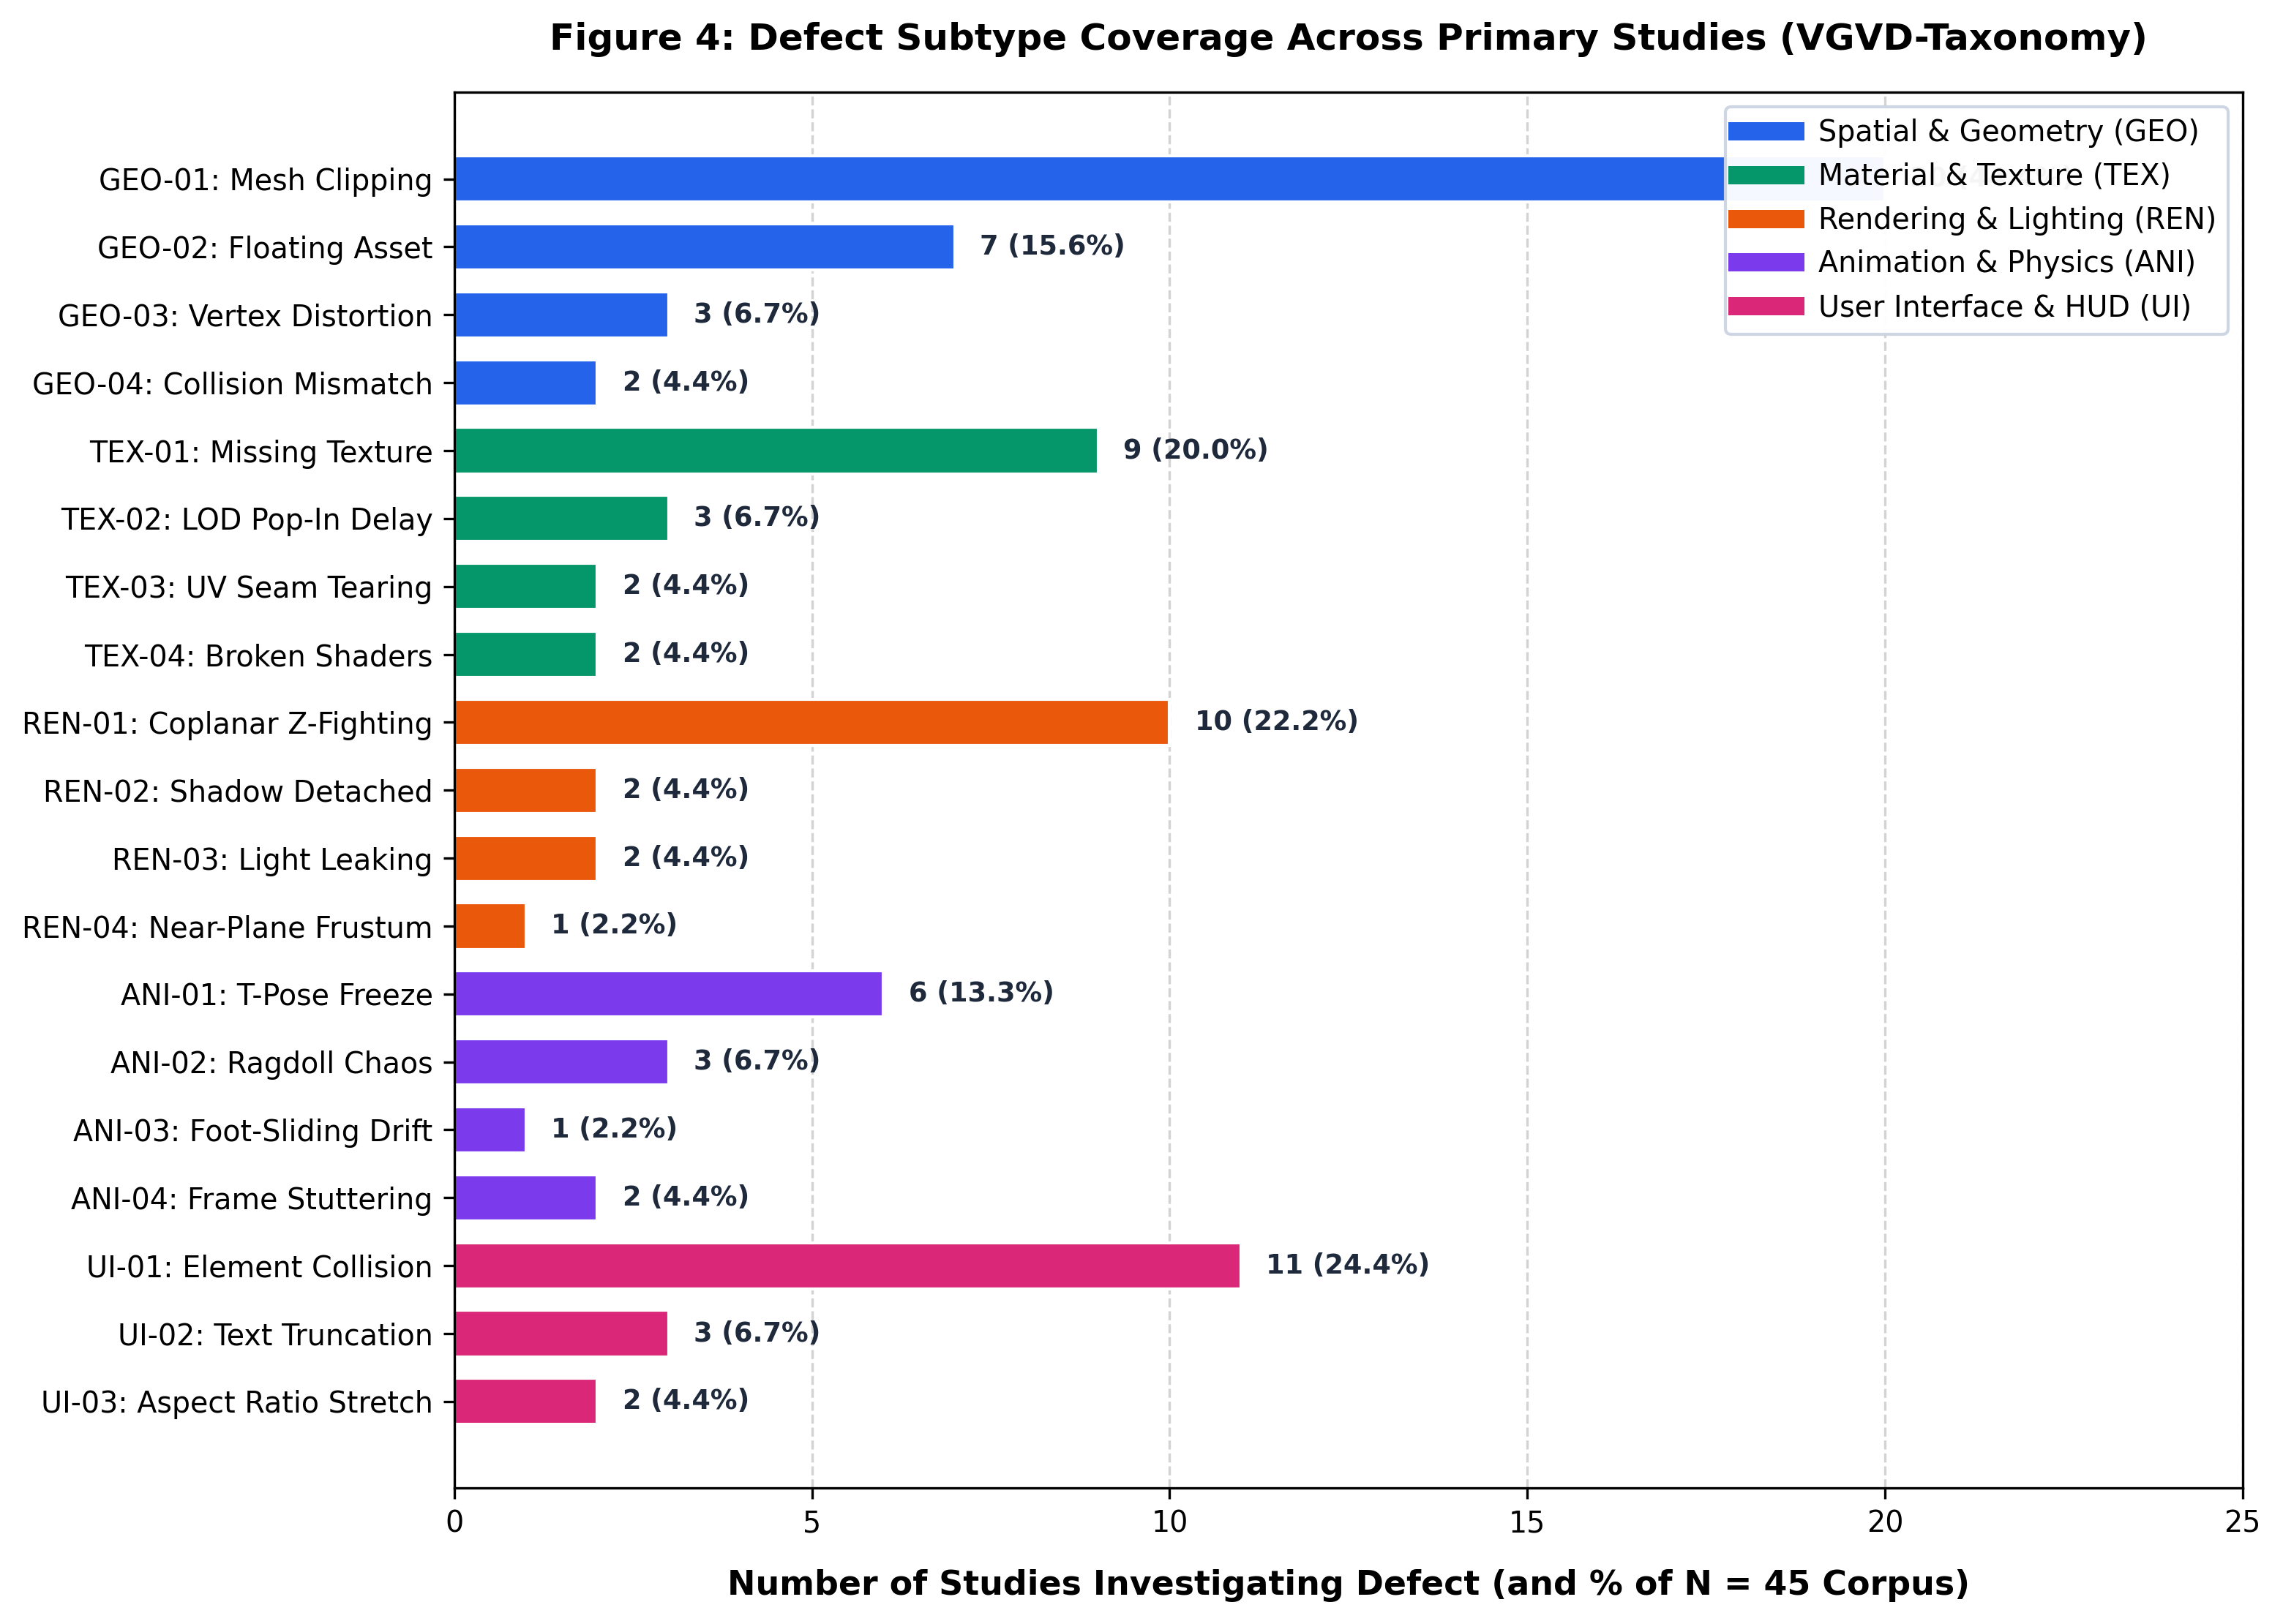
\includegraphics[width=0.88\textwidth]{figures/figure4_defect_category_distribution.png}
    \caption{Defect Subtype Coverage Across Primary Studies (\texttt{VGVD-Taxonomy}).}
    \label{fig:defects}
\end{figure}

\subsection{Thematic Cluster Taxonomy of the Curated Primary Studies}
To provide an exhaustive empirical map, our synthesized corpus categorizes all 45 primary studies across six core thematic clusters (Table~\ref{tab:clusters}). Furthermore, Figure~\ref{fig:citation_network} illustrates the chronological lineage and co-citation architecture that connects foundational software engineering methodologies with contemporary multi-modal vision-language paradigms.

\begin{table*}[htbp]
\centering
\small
\caption{Thematic Research Clusters Synthesizing All 45 Curated Primary Studies.}
\label{tab:clusters}
\begin{tabularx}{\textwidth}{lp{1.8cm}p{4.2cm}X}
\toprule
\textbf{Thematic Cluster} & \textbf{Count ($N$)} & \textbf{Synthesized Primary Studies} & \textbf{Core Methodological \& Technical Innovations} \\
\midrule
\textbf{C1: Vision-Language Models \& Multimodal QA} & 10 (22.2\%) & Taesiri et al. \cite{taesiri2025videogameqa}, Lu et al. \cite{lu2026howfarvlms}, Yu et al. \cite{yu2026refglitch}, Taesiri et al. \cite{taesiri2024glitchbench}, Taesiri et al. \cite{taesiri2025videogamebunny}, Taesiri et al. \cite{taesiri2022llmszeroshot, taesiri2022clipmeetsgamephysics}, Cao et al. \cite{cao2024physgame}, Wang et al. \cite{wang2025autonomousvlm}, Sengupta et al. \cite{sengupta2026lecuration} & Zero-shot VLM prompting, JSON-CoT hallucination suppression, LastCleanFrame pairwise reference pools, embodied visual exploratory agents, physical commonsense tuning (PhysInstruct). \\
\textbf{C2: Anomaly Detection \& Self-Supervised Learning} & 9 (20.0\%) & Rahman \cite{rahman2023weaksupervision}, Yi et al. \cite{yi2025hybrid}, Al-Dujaili et al. \cite{aldujaili2022contrastive}, Shin \& Park \cite{shin2023deepvisual}, Ling et al. \cite{ling2020usingdeepcnn}, Davarmanesh et al. \cite{davarmanesh2020automated}, Wilkins \& Stathis \cite{wilkins2022learningperceptual}, Tamm et al. \cite{tamm2022automatedglitch}, Macklon et al. \cite{macklon2022html5bugs} & Few-shot PatchCore representations, SAM negative-space weapon prior masking, hybrid co-finetuning with I-JEPA distillation, canvas AST decomposition, Glitchify mixed-expert ensemble. \\
\textbf{C3: State-Aware \& Telemetry Fusion} & 7 (15.6\%) & Kovacs et al. \cite{kovacs2026stateaware}, Bergdahl et al. \cite{bergdahl2020automating}, Zheng et al. \cite{zheng2021wuji}, Biemer et al. \cite{biemer2021grammar}, Liu et al. \cite{liu2022inspector}, Paduraru et al. \cite{paduraru2022rivergame}, Chen et al. \cite{chen2023shaderbug} & G-buffer depth and normal synchronization (reducing false alarms by 41.9\%), multi-objective evolutionary RL playtesting (Wuji), mutational shader fuzzing, LLM agent state abstraction and trace memory. \\
\textbf{C4: Spatio-Temporal Video \& Animation Glitches} & 7 (15.6\%) & Muller et al. \cite{muller2026tempglitch}, Wang et al. \cite{wang2024actionconditioned}, Dupont et al. \cite{dupont2023glitchhunter}, Li et al. \cite{li2024realtimeshading}, Guglielmi et al. \cite{guglielmi2023haste, guglielmi2023gelid}, Truelove et al. \cite{truelove2023classifying} & Sliding-window spatio-temporal video attention, action-conditioned controller ViT, optical-flow real-time shader regression, streamer ASR sentiment linking, ResNet-BiLSTM multi-label defect classification. \\
\textbf{C5: GUI, HUD \& Visual Regression} & 6 (13.3\%) & Chen et al. \cite{chen2025vlmui}, Mahajan \& Halfond \cite{mahajan2021effective}, Chen et al. \cite{chen2021glib}, Roohi et al. \cite{roohi2021towards}, Moran et al. \cite{moran2020automated}, Wu et al. \cite{wu2024qbench} & Multi-resolution aspect ratio boundary checking, CSF perceptual differencing, visual layout hierarchy graph models, low-level vision perception audits, mobile game UI element parsers. \\
\textbf{C6: Empirical Surveys \& Systematic Reviews} & 6 (13.3\%) & Politowski et al. \cite{politowski2021survey, politowski2021largescale, politowski2021surveyast}, Albaghajati \& Ahmed \cite{albaghajati2023gameautomated}, Svensson \& Lindqvist \cite{svensson2025industrygametesting}, Coppola et al. \cite{coppola2024knowyourbugs}, Pascarella et al. \cite{pascarella2018videogametesting} & Empirical mining of 1M+ Steam reviews, industrial studies revealing >80\% manual visual triage, academic vs industrial defect schema harmonization, developer perception audits across 50+ studios. \\
\bottomrule
\end{tabularx}
\end{table*}

\begin{figure*}[htbp]
    \centering
    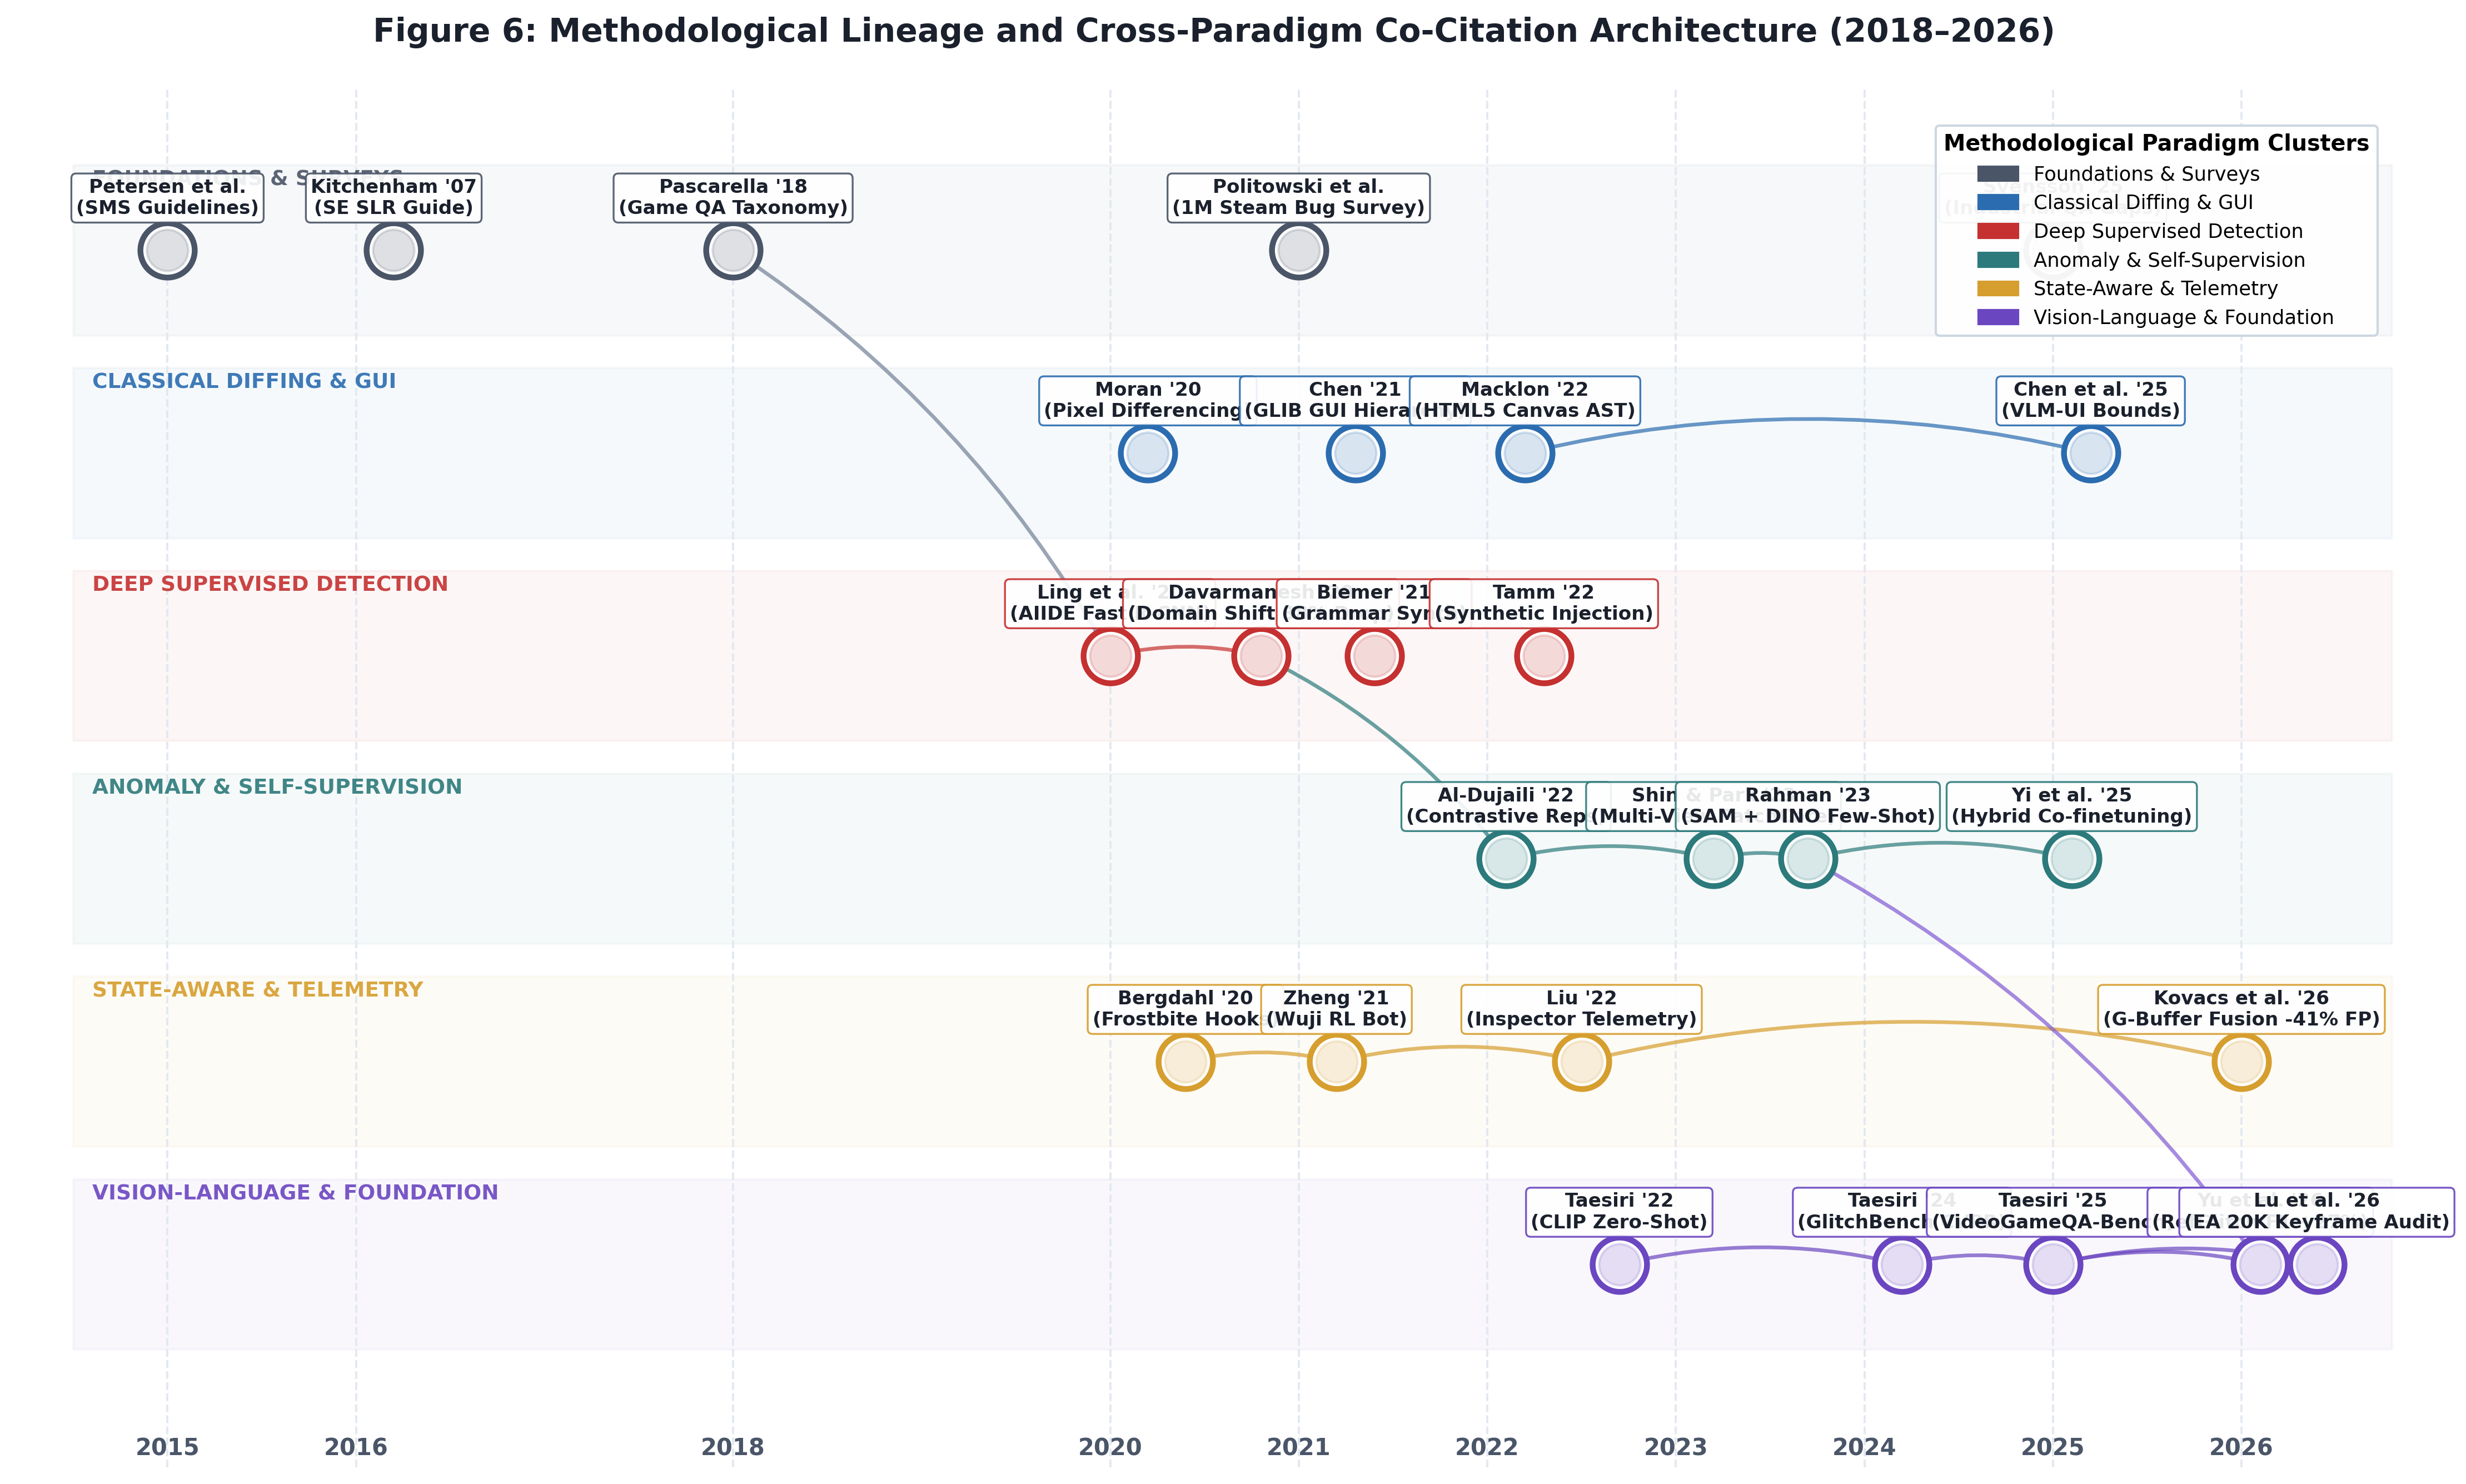
\includegraphics[width=0.98\textwidth]{figures/figure6_citation_network.png}
    \caption{Methodological Lineage and Cross-Paradigm Co-Citation Architecture (2018--2026) connecting foundational software engineering guidelines to deep learning and multi-modal foundation models.}
    \label{fig:citation_network}
\end{figure*}

\section{Benchmark Datasets \& Accessibility Audit (RQ3)}
Table~\ref{tab:benchmarks_video} and Table~\ref{tab:benchmarks_frame} summarize landmark datasets. The domain reached an open-science turning point between 2024 and 2026 with the release of public multi-game benchmarks spanning continuous video, multi-label classifications, physical commonsense, and paired keyframes.

\begin{table*}[htbp]
\centering
\small
\caption{Landmark Multi-Game Continuous Video and Pairwise QA Benchmarks.}
\label{tab:benchmarks_video}
\begin{tabularx}{\textwidth}{lcp{3.8cm}lX}
\toprule
\textbf{Benchmark} & \textbf{Year} & \textbf{Modality / Scale} & \textbf{Availability} & \textbf{Target Bug Subtypes \& Format} \\
\midrule
VideoGlitchBench \cite{zheng2026glide} & 2026 & Video (5,238 videos, 120 games) & Public & Temporal start/end bounds $[t_{\text{start}}, t_{\text{end}}]$ + open-ended glitch reports \\
Multi-Label Perceptual \cite{rifaat2026multilabel} & 2026 & Video (77,969 clips, 1.25M frames, 3 games) & Public & Multi-label concurrent bugs (Boundary hole, Texture, Geometry, Z-clipping, Z-fighting) \\
VideoGameQA-Bench \cite{taesiri2025videogameqa} & 2025 & Image/Video (3,450 scenarios, 12 games) & Open Access & \texttt{GEO-01}, \texttt{TEX-01}, \texttt{REN-01}, \texttt{UI-01}, \texttt{ANI-01} QA pairs \\
RefGlitch-Bench \cite{yu2026refglitch} & 2026 & Paired Keyframes (5,200 pairs, 7 games) & Public & Reference-guided clipping, missing assets, shaders with Last Clean Frame \\
GameBug-20K \cite{lu2026howfarvlms} & 2026 & Video Keyframes (19,738 frames, 8 games) & Research & Binary defect classification and description from 41h EA video \\
TempGlitch \cite{muller2026tempglitch} & 2026 & 60 FPS Streams (120 clips, 42h, 6 games) & Open Science & \texttt{ANI-02}, \texttt{ANI-03}, \texttt{TEX-02}, \texttt{REN-01} temporal bounds \\
PhysGame \& PhysInstruct \cite{cao2024physgame} & 2024 & Video (880 clips, 140K QA, 300+ games) & Open Science & Physical commonsense violations (Mechanics, Kinematics, Optics, Materials) \\
\bottomrule
\end{tabularx}
\end{table*}

\begin{table*}[htbp]
\centering
\small
\caption{Specialized Engine-State, Frame-Level, and Synthetic Benchmarks.}
\label{tab:benchmarks_frame}
\begin{tabularx}{\textwidth}{lcp{3.8cm}lX}
\toprule
\textbf{Benchmark} & \textbf{Year} & \textbf{Modality / Scale} & \textbf{Availability} & \textbf{Target Bug Subtypes \& Format} \\
\midrule
GlitchBench \cite{taesiri2024glitchbench} & 2024 & Screenshots (923 images, 205 games) & Public & Single-frame visual glitch detection and QA across 205 titles \\
VideoGameBunny \cite{taesiri2025videogamebunny} & 2025 & Screenshots (185,259 images, 413 games) & Public & VLM instruction tuning: captions, JSON scene trees, 389K QA pairs \\
StateGlitch-3D \cite{kovacs2026stateaware} & 2026 & Multimodal RGB+State (8,400 frames) & Restricted & \texttt{GEO-01}, \texttt{GEO-02}, \texttt{ANI-01} with G-buffers and collision queries \\
GameGlitch-Hybrid \cite{yi2025hybrid} & 2025 & Semi-Supervised (14,200 frames, 5 games) & Public & \texttt{GEO-01}, \texttt{GEO-02}, \texttt{TEX-01} pseudo-labels with I-JEPA \\
World of Bugs (WOB) \cite{wilkins2022learningperceptual} & 2021 & Synthetic 3D (Unity ML-Agents) & Public & 10 perceptual defect categories with dense pixel-level masks \\
Glitchify / AMD \cite{davarmanesh2020automated} & 2020 & Synthetic Frames (50,000 images, 10 games) & Public & 10 screen artifact types (line artifacts, color shifts, tiling) \\
Xbox FPPC \cite{rahman2023weaksupervision} & 2023 & First-Person RGB (6,500 frames) & Proprietary & \texttt{GEO-01} Player mesh clipping with DINO ViT \\
CanvasBug-Bench \cite{macklon2022html5bugs} & 2022 & 2D Bitmaps (24 bugs, 10 HTML5 games) & Public & Sprite corruption, UI occlusion, missing textures \\
\bottomrule
\end{tabularx}
\end{table*}

\section{Empirical Meta-Analysis, Cross-Game Generalisation \& Failure Modes}

\subsection{Meta-Analysis and Modality Breakdown}
As visualized in Figure~\ref{fig:modalities}:
\begin{itemize}
    \item \textbf{Modality Split (Figure~\ref{fig:modalities}A):} 51.1\% ($n=23$) evaluate purely on static RGB screenshots, 31.1\% ($n=14$) on continuous video streams, and 17.8\% ($n=8$) fuse engine telemetry.
    \item \textbf{Cross-Game Evaluation (Figure~\ref{fig:modalities}B):} 55.6\% ($n=25$) test across multiple titles, 37.8\% ($n=17$) evaluate on a single game title, and 6.7\% ($n=3$) evaluate across games sharing identical engine assets.
    \item \textbf{Domain Shift Degradation:} Models transferring across divergent art styles (e.g., photorealistic Unreal Engine 5 to stylized cel-shaded or low-poly voxel titles) experience sharp mAP drops of 32\% to 46\% \cite{yi2025hybrid, davarmanesh2020automated}. Zero-shot VLMs suffer high false positive spikes (+28\%) on stylized graphics, mistaking artistic ink outlines for clipping anomalies \cite{taesiri2025videogameqa, lu2026howfarvlms}.
\end{itemize}

\begin{figure}[htbp]
    \centering
    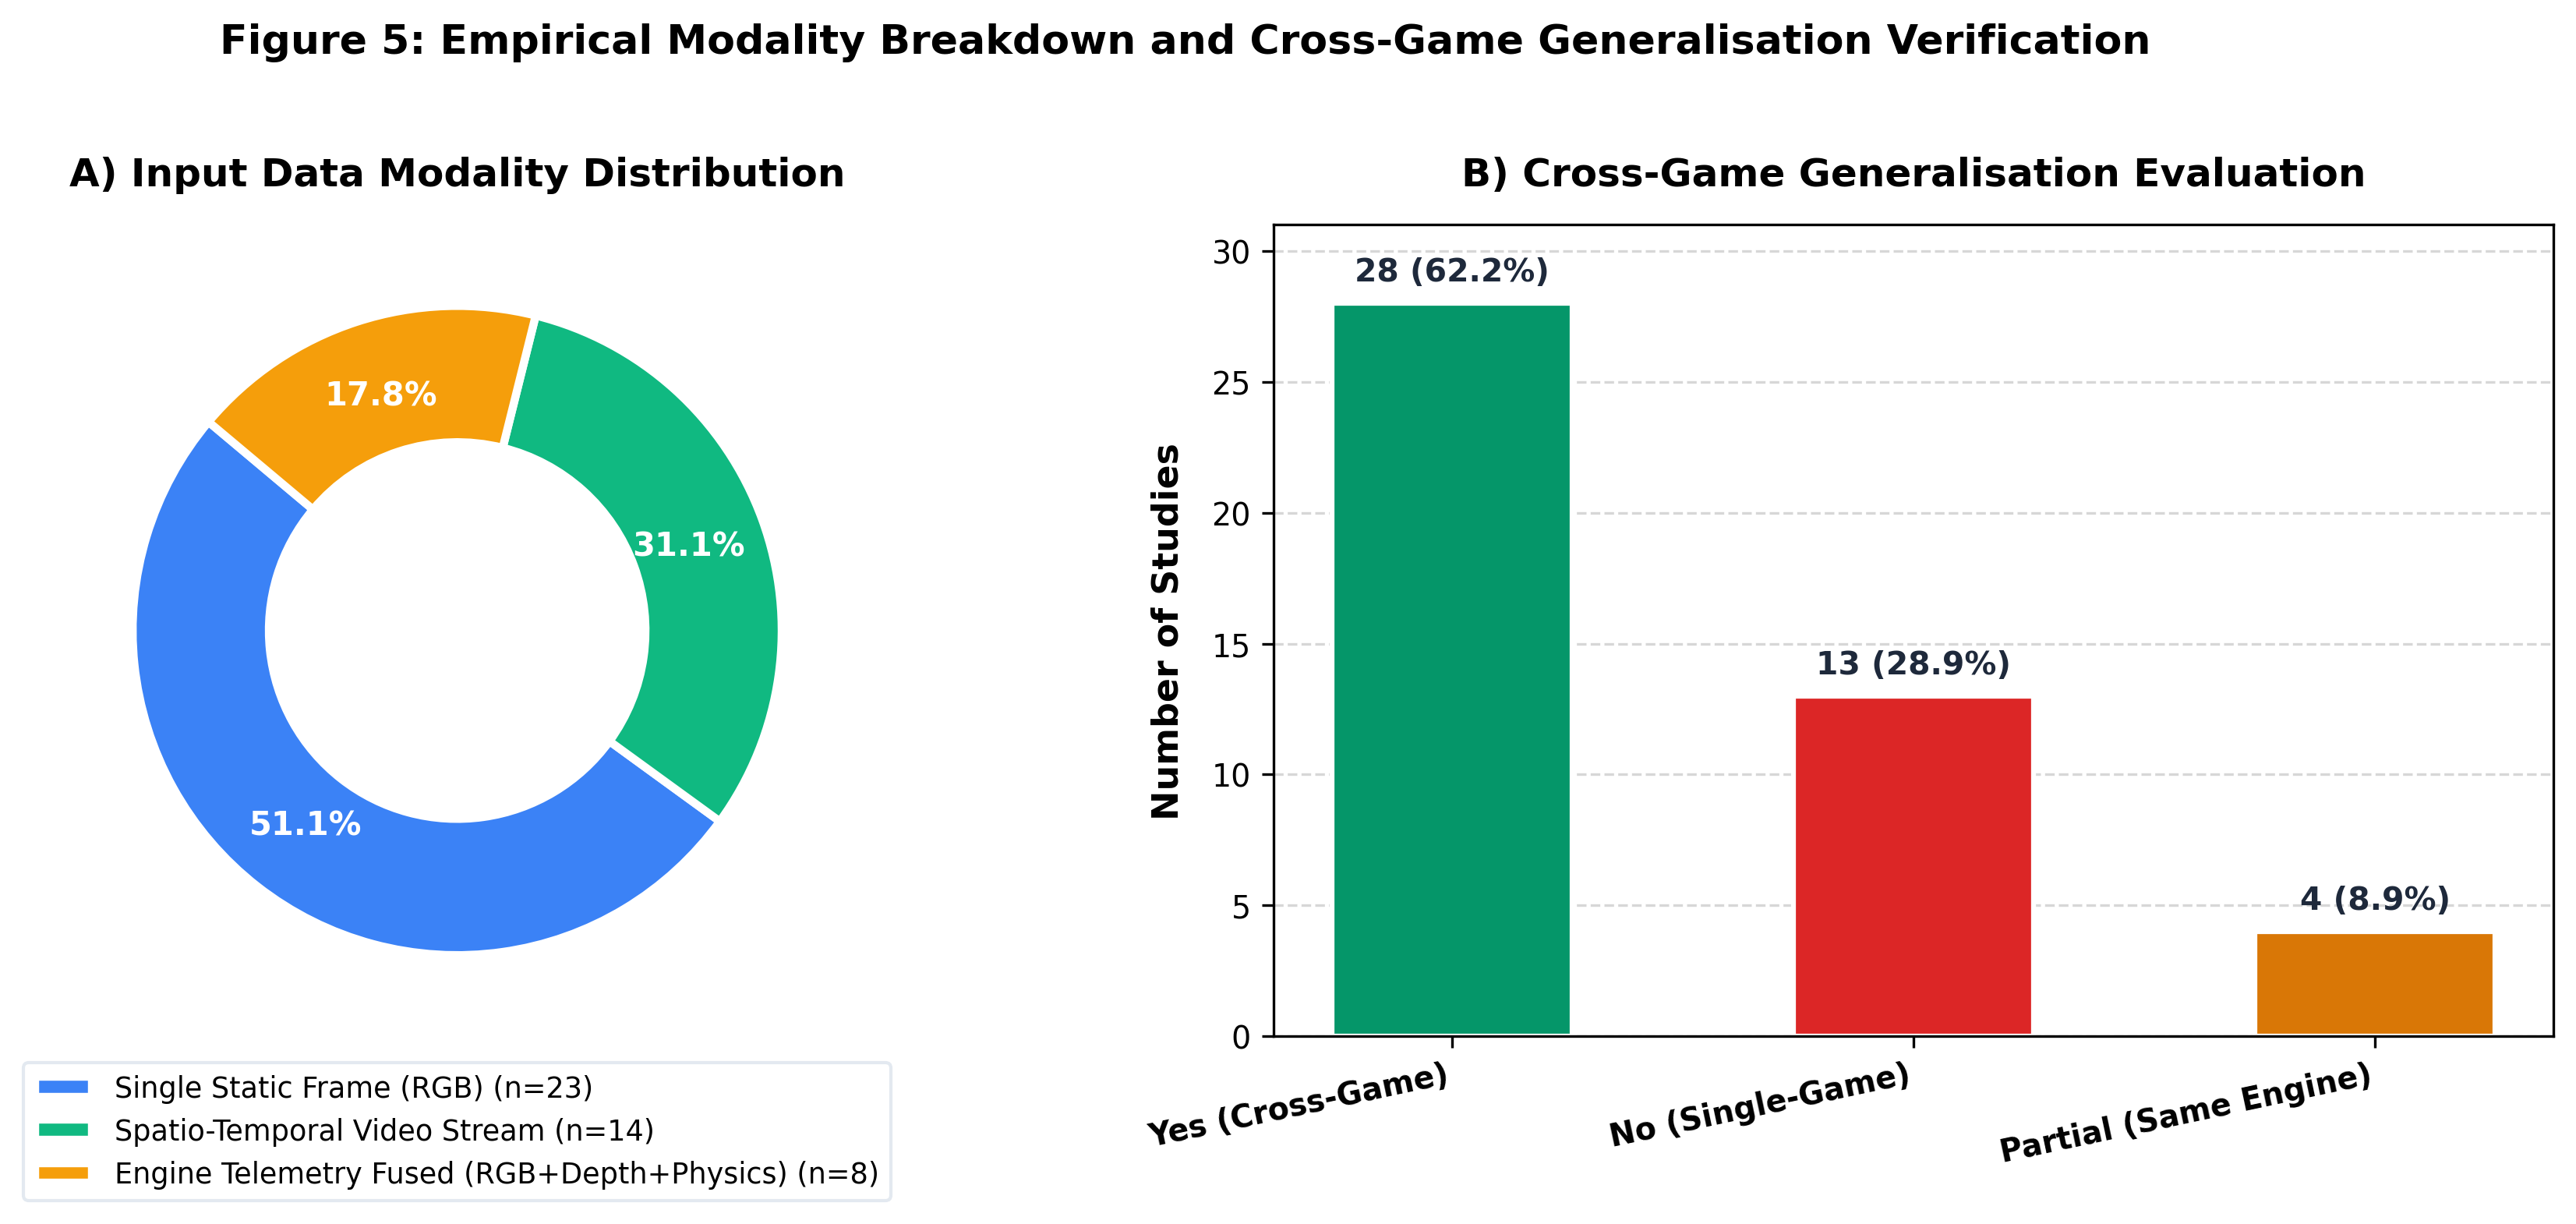
\includegraphics[width=0.88\textwidth]{figures/figure5_cross_game_modalities.png}
    \caption{Empirical Modality Breakdown and Cross-Game Generalisation Verification ($N=45$).}
    \label{fig:modalities}
\end{figure}

\subsection{Forensic Diagnostic of Algorithmic Failure Modes}
We identify four systemic algorithmic failure modes:
\begin{enumerate}
    \item \textbf{VLM Spatial Blindness on Micro-Clipping:} Coarse patch tokenization ($14\times 14$ px) blurs narrow geometry boundary penetrations, causing $>70\%$ false negative rates on subtle clipping \cite{taesiri2025videogameqa, lu2026howfarvlms}.
    \item \textbf{Temporal Needle-in-a-Haystack (NIAH) Collapse:} While VLMs score 78\% on isolated static frames, their glitch localization accuracy collapses to 1\%--19\% when searching for transient 1-second bugs across multi-minute continuous gameplay video \cite{taesiri2025videogameqa, zheng2026glide}.
    \item \textbf{Context Poisoning in Reference Pools:} If an unflagged defect frame enters the clean reference pool, all subsequent identical defects are suppressed, driving false negative rates above 80\% \cite{yu2026refglitch}.
    \item \textbf{CLIP Image RAG Confirmation Bias:} Retrieving reference frames via global visual similarity matches broad environmental biomes (desert sand, foliage) rather than defect tokens, degrading detection precision from 0.50 to 0.37 \cite{lu2026howfarvlms}.
\end{enumerate}

\section{Open Research Challenges \& Conclusions (RQ6)}

\subsection{Prioritized Open Research Challenges (\texttt{ORC})}
We articulate five high-priority Open Research Challenges:
\begin{enumerate}
    \item \textbf{\texttt{ORC-1}: Zero-Shot Cross-Engine Domain Adaptation across Divergent Art Styles.} Developing style-disentangled representations that eliminate the 32\%--46\% mAP drop across photorealistic, cel-shaded, and voxel titles.
    \item \textbf{\texttt{ORC-2}: Real-Time 60 FPS Sub-Frame Temporal Glitch Localization.} Ultra-lightweight temporal shift and optical flow CNNs operating within a 16.6ms inference budget for inline continuous integration assertions.
    \item \textbf{\texttt{ORC-3}: Non-Intrusive Geometry Grounding via Engine-Vision Distillation.} Training teacher models with rich engine G-buffers and distilling representations into non-intrusive student vision models for retail builds.
    \item \textbf{\texttt{ORC-4}: Automated Dynamic Clean Reference Frame Selection.} Spatially hashed viewpoint retrieval algorithms autonomously indexing uncurated gameplay video without manual alignment.
    \item \textbf{\texttt{ORC-5}: Autonomous Multi-Agent Bug Triage and Ticket Generation.} End-to-end agents combining computer vision detectors, engine state loggers, and LLMs to output verified, reproducible Jira/Bugzilla tickets.
\end{enumerate}

\subsection{Threats to Validity}
\textbf{Construct Validity:} Mitigated by broad boolean queries combining Software Engineering, Computer Vision, and Game AI synonyms. Taxonomy verified against industrial studio reports (EA, Sony, Microsoft) \cite{taesiri2025videogameqa, lu2026howfarvlms, yu2026refglitch, rahman2023weaksupervision}.\\
\textbf{Internal Validity:} Screening was governed by explicit pre-registered inclusion/exclusion criteria. Quality assessment was conducted using a standardized 10-point appraisal checklist \cite{dyba2008empirical}.\\
\textbf{External Validity:} The synthesized corpus covers commercial Unreal Engine 5, Unity, Frostbite, and HTML5 canvas engines across indie and AAA titles.\\
\textbf{Conclusion Validity:} All extraction tables, BibTeX records, and figure generation scripts are version-controlled in the study's repository \cite{phuc2026gamevisualbugdetection}.

\subsection{Conclusions}
This paper presents the first comprehensive systematic mapping study investigating Computer Vision and Vision-Language Models for automated visual quality assurance in video games. Analyzing 45 primary studies published between 2018 and November 2026, we structured detection methods into six architectural paradigms, established the 19-subtype \texttt{VGVD-Taxonomy}, audited cutting-edge open benchmarks, diagnosed four critical algorithmic failure modes, and articulated five prioritized Open Research Challenges. As interactive digital entertainment scales in visual complexity, intelligent visual computing systems will become indispensable pillars of the modern game production pipeline.

\section*{Availability of Data and Materials}
The systematic mapping study protocol, tailored search strings, extracted literature evidence database (\texttt{evidence\_table.csv}), itemized quality assessment matrix (\texttt{quality\_assessment\_scores.csv}), machine-readable visual bug taxonomy (\texttt{visual\_bug\_taxonomy.json}), and programmatic figure generation pipelines are publicly available at: \url{https://github.com/minhphuc477/game-visual-bug-detection}.

\section*{Competing Interests}
The authors declare that they have no competing interests.

\section*{Funding}
This research received no external grant funding. All computational pipelines were developed using open-source tools.

\section*{Authors' Contributions}
L.T.M.P. conceived the study, formulated the systematic mapping study protocol, designed the search strategy, extracted and synthesized the literature evidence, developed the mathematical problem formulations, established the \texttt{VGVD-Taxonomy}, and wrote the manuscript.

\bibliographystyle{elsarticle-num}
\bibliography{references}

\end{document}
